\documentclass[a4paper,overfullrule=true,9pt]{scrartcl}

% Uncomment to optimize for double-sided printing.
% \KOMAoptions{twoside}

% Set binding correction manually, if known.
% \KOMAoptions{BCOR=2cm}

% Typographic niceties fixing a multitude of potential small issues
\usepackage{microtype}

% Localization options
\usepackage[english]{babel}
\usepackage[T1]{fontenc}
\usepackage[utf8]{inputenc}

% \hyph to allow hyphen which doens't break auto-hyphenation
\usepackage{hyphenat}

% Custom hyphenation
\hyphenation{dis-car-ded re-sul-ted ka-na-my-cin plas-mids trea-ted co-lo-nies mem-branes over-night fluo-res-cence ali-quots clea-ved un-clea-ved Chlor-am-phe-ni-col quen-ched me-di-um}


% Reset section numbers within each part
\usepackage{chngcntr}
\counterwithin{section}{part}
% Use arabic numerals for parts (rather than default roman ones)
\renewcommand{\thepart}{\arabic{part}}

% Number headings until level 2 (subsections)
\setcounter{secnumdepth}{2}

% Quotations
\usepackage{dirtytalk}

% Enhanced verbatim sections. We're mainly interested in
% \verbatiminput though.
\usepackage{verbatim}

% PDF-compatible landscape mode.
% Makes PDF viewers show the page rotated by 90°.
\usepackage{pdflscape}

% Subfigures
\usepackage{subcaption}

% Figures at end (of chapter via \processdelayedfloats)
% \usepackage[figuresonly,nomarkers,nofiglist]{endfloat}

% minitables but with variable width
\usepackage{varwidth}

% Advanced tables
\usepackage{tabu}
\usepackage{longtable}

% Fancy tablerules
\usepackage{booktabs}

% Graphics
\usepackage{graphicx}

% Current time
\usepackage[useregional=numeric]{datetime2}

% Float barriers.
% Automatically add a FloatBarrier to each \section
\usepackage[section]{placeins}

% Importing CSV into tables
\usepackage{csvsimple}

\usepackage{geometry}
\usepackage{layout}

% Math tools
\usepackage{mathtools}
% Math symbols
\usepackage{amsmath,amsfonts,amssymb}
\usepackage{amsthm}

\DeclarePairedDelimiter\abs{\lvert}{\rvert}

\pagestyle{plain}
 
% Source code & highlighting
\usepackage{listings}

% SI units
\usepackage[binary-units=true]{siunitx}
\DeclareSIUnit\Molar{\textsc{m}}
\DeclareSIUnit\Da{Da}
\DeclareSIUnit\mole{mol}
\DeclareSIUnit\rpm{rpm}
\DeclareSIUnit\cfu{cfu}
% Uncertainity as separate value
\sisetup{separate-uncertainty}

\usepackage[version=4]{mhchem}

\newcommand{\odbact}{$\text{OD}_{600}$}
\newcommand{\ecoli}{\textit{E. Coli}}
\newcommand{\hs}{cybB561}
\newcommand{\hsmut}{\hs-H158F}
\newcommand{\hsdsred}{\hs-Dsred}

\newcommand{\mysubject}{2115 - Lab course biochemistry 2}
\newcommand{\mytitle}{Expression, purification and characterization of superoxide oxidase SOO}

% Convenience commands
\newcommand{\mailsubject}{\mysubject{} \mytitle{}}
\newcommand{\maillink}[2]{\href{mailto:#1?subject=\mailsubject}
                               {#2}}

% Should use this command wherever the print date is mentioned.
\newcommand{\printdate}{\today}

\subject{2115 - Lab course biochemistry 2}
\title{Expression, purification and characterization of superoxide oxidase `SOO'}
\subtitle{Final report}
\author{\maillink{michael.senn@students.unibe.ch}{Michael Senn} - 16-126-880}

\date{\printdate}

\publishers{von Ballmoos group, University of Bern\\Abbas Maxime Abou Hamdan \& Sabina Deutschmann}

% Needs to be the last command in the preamble, for one reason or
% another. 
\usepackage{hyperref}

\begin{document}
\maketitle

\begin{abstract}
	Three variants of \ecoli{} superoxide oxidase were grown in bacterial
	BL21 cells and purified using size-exclusion and affinity
	chromatography.  Purification efficiency was monitored using
	fluorescence of dsRed-tagged proteins.

	Purified enzymes were reconstituted into liposomes using freeze-thaw
	cycles. Orientation of proteins in reconstituted liposomes was analysed
	by TEV-cleaving and fluorescence measurements. 

	Reduction of reconstituted and solubilized enzymes was measured in
	presence of superoxide or quinol via absorbance measurements, as well
	as its enzymatic activity in a WST-1 assay containing sources of
	quinone and superoxide.

	Using the collected data the enzymes were characterised, estimating
	their $K_m$ value as well as gaining insights into the orientation of
	enzymes in liposomes.
\end{abstract}

\part{Introduction}

Reactive oxygen species (`ROS') such as superoxide (\ce{O2-}) or hydrogen
peroxide (\ce{H2O2}) are toxic to the body, causing damage to proteins or DNA,
with links to various diseases including cancer. As such organisms under
aerobic conditions counteract ROS via eg Superoxide Dismutase (`SOD') which
catalyzes the partitioning of superoxide into molecular oxygen and hydrogen
peroxide.

One major source of superoxide is the oxidative phosphoryliation within the
mitochondrial matrix. \cite{Novo2008} To a lesser extent these superoxides
diffuse into the cytoplasm, where they are acted upon by SOD. A significant
portion of superoxides however is oxidised by superoxide oxidases - henceafter
referred to as `SOO' or `Halonsaft' due to its colour - a family of
membrane-bound proteins which oxidize superoxides.\cite{superoxide_salvaging}.

One protein of this family is CybB from \ecoli{} which was shown to function as
a superoxide:ubiquinone oxidoreductase. It oxidizes superoxide to oxygen while
simultaneously reducing quinone to quinol.\cite{superoxide_salvaging} This
enzymatic activity both serves to remove superoxides in close proximity to the
cell membrane, as well as restore the quinone pool, helping to save energy.

% TODO
% - Characterizing (eg activity) we did?
% - Transformation & expression basics
% - Which mutation (H158F)


\twocolumn

\part{Material \& methods}

\section{Transformation \& expression}

\small

Transformation and expression were done as described.
\cite{superoxide_salvaging}. Summarily, \ce{CaCl2} treated cells were mixed
with pET28-cybB561 plasmids, and heat shock treated (\SI{30}{\min} on ice,
\SI{1}{\min} at \SI{42}{\celsius}, \SI{5}{\min} on ice, \SI{1}{\hour} at
\SI{37}{\celsius} shaking at \SI{900}{rpm}), then incubated overnight at
\SI{37}{\celsius} with \SI{30}{\ug\per\ml} Kanamycin. Transformed colonies were
picked and incoluated overnight at \SI{37}{\celsius} in LB medium with
\SI{30}{\ug\per\ml} Kanamycin and \SI{35}{\ug\per\ml} Chloramphenicol.

% TODO: Antibiotic amounts correct? Check lab journal

\section{Membrane isolation \& enzyme purification}

Purification of SOO was done as described. \cite{superoxide_salvaging}.

In summary, resuspended bacterial cells were broken open and DNASE-treated in a
maximator (3 passes at $>$\SI{1000}{\bar}). Pelleted membranes were resuspended
in \SI{50}{\milli\Molar} HEPES pH 7.5, \SI{200}{\milli\Molar} \ce{NaCl},
\SI{7.5}{\percent} glycerol buffer. Protein concentration was determined with a
BCA assay.

Membranes were solubilized in \SI{1}{\percent} OGNG \SI{1}{\milli\Molar} PMSF
and stirred at \SI{4}{\celsius} for \SI{1}{\hour}. Insolubilized membranes were
pelleted at \SI{150000}{g} for \SI{45}{\min}. The supernatant was loaded on a
\ce{Ni^{2+}} column and incubated for \SI{45}{\min} at \SI{4}{\celsius} on a
rotating wheel. The column was then washed and eluted with \SI{5}{\milli\Molar}
and \SI{100}{\milli\Molar} Histidine.

Parts of cybB561-dsRed were treated overnight with TEV-protease, and a reverse
\ce{Ni^{2+}} IMAC performed.

The eluate was concentrated to \SI{0.5}{\ml} with a \SI{10}{\kilo\Da}
concentrator, and loaded onto a S200 increase 10/300 column. Fractions
suspected to contain the protein were pooled. Protein concentration was
determined via absorbance mesurement of oxidized and reduced form (via addition
of DTT) between \SIrange{600}{400}{\nm}.

Aliquots of the purification steps were loaded onto a \SI{12}{\percent}
SDS-PAGE gel, ran at \SI{125}{\V} for \SI{20}{\min} and \SI{185}{\V} for
\SI{80}{\min}. The gel was stained with coomassie.

Efficiency of purification was measured via fluorescence measurement of
cyB561-dsred at an emission of \SI{586}{\nm} and extinction of \SI{555}{\nm}.

\section{Enzyme characterization}

Characterization was performed according to the same Nature
article\cite{superoxide_salvaging}.

Dried lipis were resuspended in \SI{20}{\milli\Molar} HEPES pH 7.4,
\SI{20}{\milli\Molar} \ce{KCl}, \SI{200}{\milli\Molar} \ce{NaCl}. Unliamellar
liposomes were formed by freeze-thaw cycles in nitrogen and \SI{29.4}{\celsius}
respectively, followed by sonication (\SI{2.5}{\min}, cycles of \SI{0.5}{\min}
on \SI{0.5}{\min} off).

CybB was reconstituted by adding enzymes to liposomes with \SI{0.6}{\percent}
sodium cholate. Detergent was removed by loading the sample on a P10 gel
filtration column and eluting it.

Reduction of CybB was measured via absorption measurement at \SI{428}{\nm}. In
a first set \SI{1}{\micro\Molar} of solubilized enzyme was mixed with
\SI{20}{\milli\Molar} HEPES ph 7.4, \SI{20}{\milli\Molar} \ce{KCl},
\SI{200}{\milli\Molar} \ce{NaCl}, \SI{0.05}{\percent} DDM for a final reaction
volume of \SI{750}{\ul}. At t=\SI{1}{\min} \SI{1}{\ul} substrate (quinol or
superoxide via Xanthyloxidase) was added, at t=\SI{3}{\min} the enzyme was
fully reduced via DTT. In a second set the same experiment was performed with
\SI{10}{\ul} reconstituted enzymes in equal fashion except a buffer without
detergent was used. The two sets were done for both the wildtype as well as the
mutant.

Fluorescence of reconstituted and solubilized, cleaved and uncleaved CybB-sred
was measured at excitation of \SI{555}{\nm} and emission of \SI{595}{\nm}.
Fluorescence was quenched with \ce{Cu2+} and restored with EDTA.

Activity of solubilized enzymes was determined by measuring reduction of WST-1
via absorption at \SI{455}{\nm}. In a first set \SI{100}{\micro\Molar} quinone,
\SI{60}{\nano\Molar} BO3 oxidase and buffer (\SI{100}{\milli\Molar} sodium
phosphate pH 8, \SI{0.1}{\milli\Molar} DTPA, \SI{0.1}{\milli\Molar}
Hypoxanthine, \SI{0.05}{\percent} DDM) for a final volume of \SI{750}{\ul} were
mixed. At t=\SI{0.5}{\min} \SI{0.03}{U} XO, at t=\SI{1.5}{\min} varying volumes
of enzyme were added. Enzyme concentration was increased until quenching of
superoxide production was level with a reference measurement done using
superoxide dismutase.

In a second set the determined concentration of enzyme was kept constant while
quinone concentration was varied.

\normalsize


\twocolumn

\part{Results \& discussion}

\section{Transformation}

The goal of bacterial transformation was to get competent \ecoli{} cells of the
LEMO21 (DE3) strain to take up pET28a-cybB561 plasmids, allowing for the
selective overexpression of HS in presence of lactose or IPTG. Rhamnose allowed
to selectively inhibit the T7 polymerase translating the HS gene.
\cite{memstar} To permit selection the plasmid further encodes for a resistance
to kanamycin.

The overnight incubated plates containing kanamycin had multiple colonies
growing on them the next day. This showed that the heat shock treatment had
been successful. Transformed colonies were not used further due to time
constraints, rather expression was monitored simultaneously with
pre-transformed starting culture.

\section{Expression}

Note that bacteria resulting from this step were not used further due to time
constraint. Rather purification happened simultaneously, with a provided
bacterial pellet.

\subsection{Expression monitoring}

During expression the efficiency of several media was to be established, both
in terms of speed of cell growth as well as yield of HS per cell. Three
different types of medium (LB, TB, ZYM-505) were prepared, with four samples
each.

Increasing the amount of produced proteins per cell was of interest as it
lowers the amount of detergent required to solubilize the cell membranes.

Protein expression was monitored by measurement of \odbact of incubating
samples, visualized in figure \ref{fig:absorption_expression}. A measurement at
\SI{90}{\min} was excluded as it had been done incorrectly. IPTG was added at
\SI{90}{\min}.

It was shown that cells grew faster in TB and ZYM-505 medium than in LB medium,
as seen by the slope of the curve as well as final \odbact reached. This was
likely caused by the higher concentration of nutrients such as yeast extract
and tryptone in the case of TB, respectively additional glucose and lactose in
the case of ZYM-505.

It was further shown that samples not containing IPTG followed the normal
growth pattern of bacterial cells, starting in a lag phase of little cell
growth, a log phase of exponential cell growth - shown as a linear increase of
\odbact - and the beginnings of a stationary phase where cell growth cedes. The
absence of IPTG will have prevented overexpression of HS, allowing cells to
grow as normal.

Cells treated with IPTG at \SI{90}{\min} and not containing Rhamnose showed
stagnation of cell growth indicative of overexpression of HS. Cells treated
with IPTG and containing Rhamnose did not show any sign of overexpression of
HS.

\subsection{Expression efficiency}

After expression the amount of expressed \hsdsred{} was measured via fluorescence
measurements. Results were normalized to cell density, giving an approximation
of protein concentration per cell. Such normalized results are are shown in
figure \ref{fig:fluorescence_expression}.

\subsubsection{Base protein expression}

Overall protein expression per cell can be estimated using IPTG-negative
samples. It was shown that LB and ZYM-505 media produce comparable amounts of
proteins per cell, while the amount of proteins per cell in the TB medium was
significantly higher. This conflicts with the memstar paper which found that
protein production normalized to cell density was only slightly higher in TB
compared to the other two media. \cite{memstar}

It is possible that the cell density of the TB samples was underestimated, as
the linear relation between \odbact and cell density only holds for low values
of \odbact, as well as the spectrophotometer being less accurate for values
exceeding $1$.

\subsubsection{\hsdsred{} expression}

Comparing the normalized fluorescence of IPTG-positive, Rhamnose-negative
samples with other samples in the same media showed that addition of IPTG
increased the amount of proteins - specifically \hsdsred{} - which was expressed
per cell.

\subsubsection{Limiting \hsdsred{} expression with Rhamnose}

Addition of Rhamnose to samples was supposed to limit the overexpression of
\hsdsred{}, preventing a complete stagnation of cell growth as well as the
potential buildup of inclusion bodies. \cite{memstar}.

As Rhamnose-positive samples did not show any sign of \hsdsred{} expression, with
fluorescence levels comparable to IPTG-negative samples, we conclude that
either too much Rhamnose was added such that the T7 polymerase was inhibited
fully, or that no IPTG had been added to those samples.


\begin{figure}
	\centering
	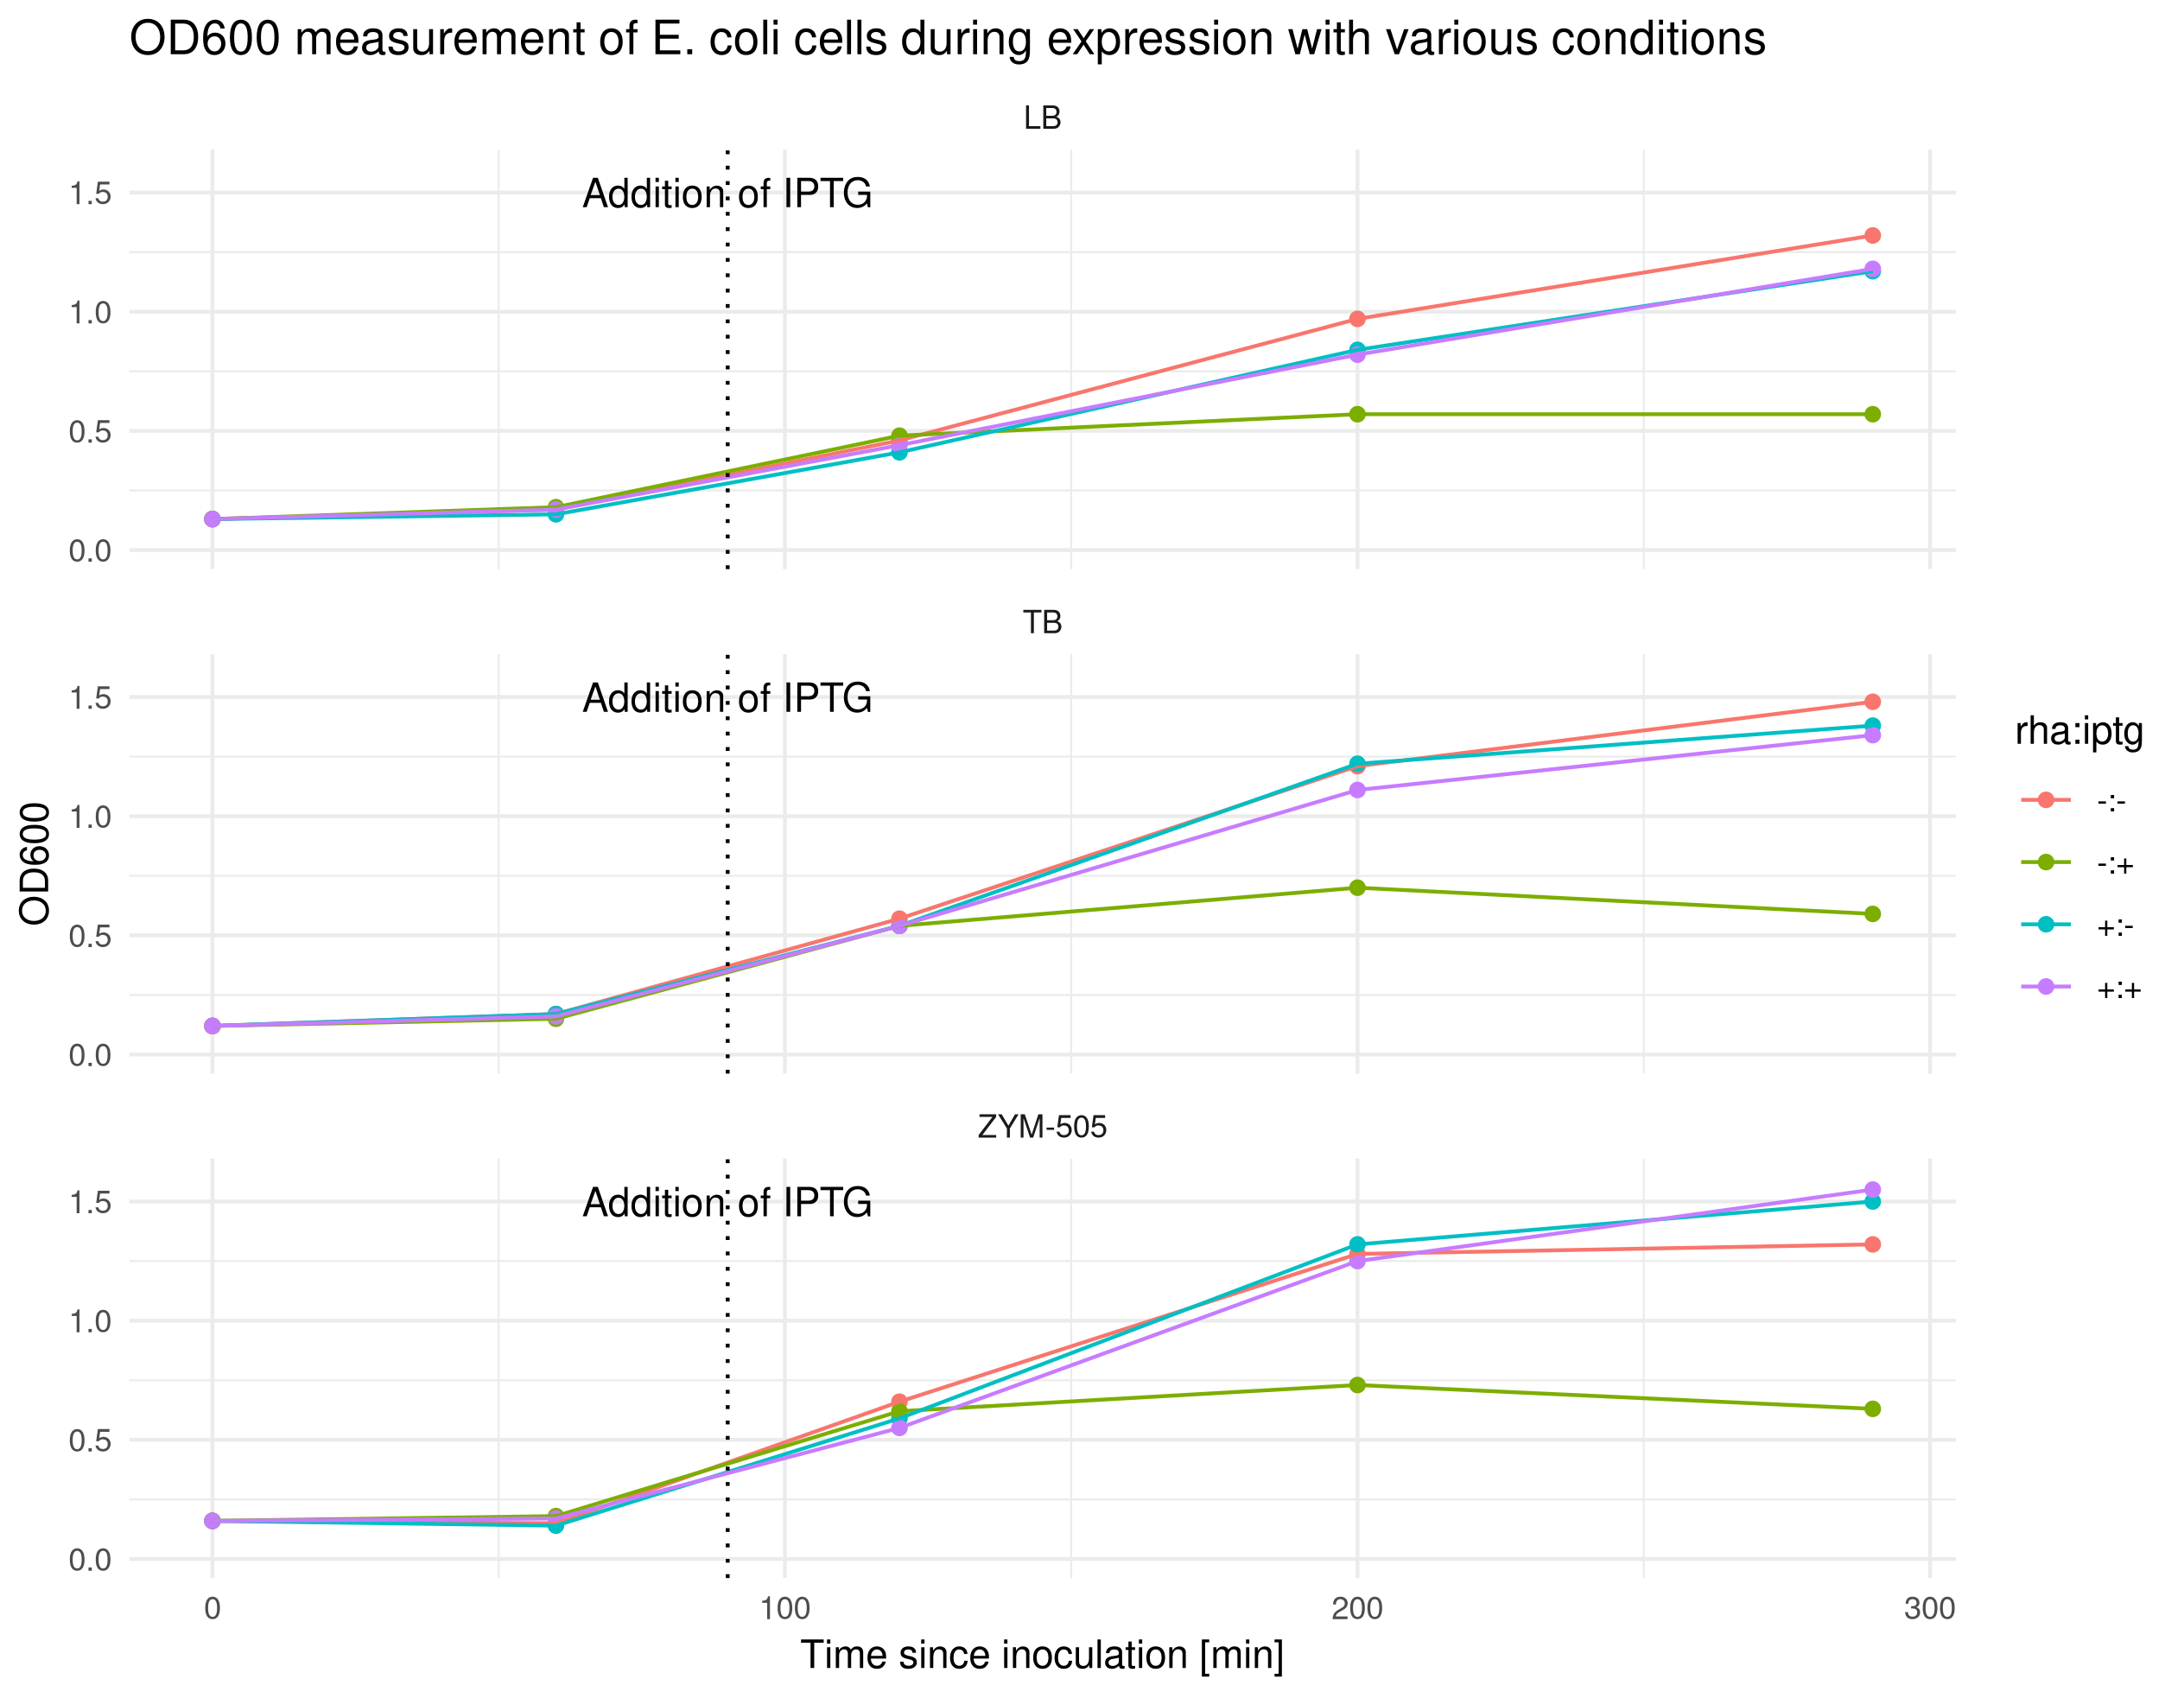
\includegraphics[width=\linewidth]{../img/absorption_expression.png}
	\caption{Monitoring expression speed via \odbact values over time}
	\label{fig:absorption_expression}
\end{figure}

\begin{figure}
	\centering
	\includegraphics[width=\linewidth]{../img/expression_fluorescence.png}
	\caption{Fluorescence of samples after protein expression}
	\label{fig:fluorescence_expression}
\end{figure}

\section{Purification}

\subsection{Membrane protein concentration}

Concentration of harvested membrane proteins was determined in a BCA assay by
comparison with a known standard. Absorption at \SI{562}{\nm} of the standard
was measured and a linear regression calculated as $\text{absorption} = 0.81542
\cdot \text{concentration} + 0.02701$. Measured absorption and calculated
concentrations of a dilution of membrane proteins are shown in table
\ref{tbl:bca_absorption_sample}.

Measurements with absorption values outside the standard's range of 0.0053 to
1.6353 were discarded, which resulted in an average protein concentration of
\SI{22.86 \pm 3.20}{\mg\per\ml}.

\begin{table*}
	\centering
	\begin{tabu}{llll}
		\toprule
		Absorption & Conc (linear regression) & Dilution factor & Conc (undiluted) \\
		\midrule
		\SI{2.3066}{OD562} & \SI{2.78}{\mg\per\ml} & 1:5  & \SI{13.92}{\mg\per\ml} \\
		\SI{1.8855}{OD562} & \SI{2.28}{\mg\per\ml} & 1:10 & \SI{22.80}{\mg\per\ml} \\
		\SI{0.8671}{OD562} & \SI{1.03}{\mg\per\ml} & 1:20 & \SI{20.60}{\mg\per\ml} \\
		\SI{0.5388}{OD562} & \SI{0.63}{\mg\per\ml} & 1:40 & \SI{25.12}{\mg\per\ml} \\
		\bottomrule
	\end{tabu}
	\caption{OD562 values of sample dilutions}
	\label{tbl:bca_absorption_sample}
\end{table*}

\subsection{Purified protein concentration}

Protein concentration was determined using the absorbance of the two hemes at
\SI{561}{\nm} as described. Measurement values between \SIrange{400}{600}{\nm}
are shown in figure \ref{fig:hs_concentration}.

A baseline was established by calculating the average absorption difference of
reduced and oxidised form between \SIrange{580}{600}{\nm}. The absorption
difference at \SI{561}{\nm} was calculated and the baseline difference added.

Given the path length of the cuvette as \SI{1}{\cm}, a dilution factor of 375
and an extinction coefficient of \SI{46.36}{\per\milli\Molar\per\cm} the
protein concentration was calculated using Beer's law. Such calculated
concentrations are shown in table \ref{tbl:hs_concentration}.

\begin{table*}[ht]
	\begin{varwidth}[b]{0.4\linewidth}
		\centering
		\begin{tabu}{ll}
			% \toprule
			% Protein & Wt & Mut & Dsred \\
			% $\Delta_{\text{OD}_{\SI{561}{\nm}}}$ & 0.042 & 0.043 & 0.068 \\
			% Baseline & 0.004 & 0.006 & 0.013 \\
			% $\Delta_{\text{OD}_{\SI{561}{\nm}\text{ corr}}}$ & 0.046 & 0.049 & 0.081 \\
			% Conc [\si{\milli\Molar}] & 0.372 & 0.397 & 0.655 \\
			% \bottomrule
			\toprule
			\multicolumn{2}{c}{\hs{}} \\
			\midrule
			$\Delta_{\text{OD}_{\SI{561}{\nm}}}$ & 0.042 \\
			Baseline & 0.004 \\
			$\Delta_{\text{OD}_{\SI{561}{\nm}\text{ corr}}}$ & 0.046 \\
			Conc [\si{\milli\Molar}] & 0.372 \\

			\midrule
			\multicolumn{2}{c}{\hsmut{}} \\
			\midrule
			$\Delta_{\text{OD}_{\SI{561}{\nm}}}$ & 0.043 \\
			Baseline & 0.006 \\
			$\Delta_{\text{OD}_{\SI{561}{\nm}\text{ corr}}}$ & 0.049 \\
			Conc [\si{\milli\Molar}] & 0.397 \\

			\midrule
			\multicolumn{2}{c}{\hsdsred{}} \\
			\midrule
			$\Delta_{\text{OD}_{\SI{561}{\nm}}}$ & 0.068 \\
			Baseline & 0.013 \\
			$\Delta_{\text{OD}_{\SI{561}{\nm}\text{ corr}}}$ & 0.081 \\
			Conc [\si{\milli\Molar}] & 0.655 \\
			\bottomrule
		\end{tabu}
		\caption{Purified HS conc.} % Must not be long enough to cause line-break, else varwidth fails
		\label{tbl:hs_concentration}
	\end{varwidth}%
	\hfill
	\begin{minipage}[b]{0.6\linewidth}
		\centering
		\includegraphics[width=\textwidth]{../img/hs_concentration.png}
		\captionof{figure}{Absorption of HS for concentration determination}
		\label{fig:hs_concentration}
	\end{minipage}
\end{table*}

\subsection{SDS PAGE}

Purification steps were checked with an SDS page, results shown in figure
\ref{fig:sds}.

\subsubsection{\hs{} \& \hsmut{}}

Cyan marks HS, with an expected molecular weight of
\SI{24}{\kilo\Da}\cite{pdb}. As was expected it was highly concentrated after
the \ce{Ni} bead chromatography, and remained so after the ÄKTA SEC.
Furthermore it can be seen in small quantities in the \SI{5}{\milli\Molar} His
wash implying that a small amount was lost when washing the column as the
His-tagged buffer displaced the His-tagged protein from the column. As the band
of the after-ÄKTA steps seems smaller than the one preceding it it is assumed
that some was also lost during the SEC.

\subsubsection{\hsdsred{}}

Green marks the \hsdsred{} pair, with a combined expected weight of
\SI{49}{\kilo\Da} \cite{pdb}. It takes the place of plain HS in the samples of
\hs{} and \hsmut{}. After TEV cleavage - that is from the `before loading'
column on onward - there is no band at this height anymore, which shows that
either cleavage was successful or \hsdsred{} was lost another way. After
cleavage the single HS is marked in cyan, near its expected size of
\SI{24}{\kilo\Da}. Of interest are faint bands on the same height in the
samples before cleavage, which might imply that a small amount of \hsdsred{}
had been cleaved before. In the reverse IMAC \hs{} was mostly found in the
flowthrough, as the His tag is on the Dsred so \hs{} was unable to bind to the
column. Small amounts can be seen in the elution, implying that an intermediary
wash step might have been required if a clean separation of \hs{} and Dsred was
desired.

Red marks Dsred with its molecular weight of \SI{25}{\kilo\Da}, further
identified by being on the same height as the pure Dsred loaded in the last
lane. It is mostly visible in the elution after cleavage, as its His tag
allowed binding to the column, with tiny amounts visible in the flowthrough. Of
interest once more were the corresponding bands in the lanes before cleavage.
These were either due to impurities of a comparable size, or small amounts of
\hsdsred were cleaved even before TEV protease was added - either due to
another protease, or due to small amounts of TEV protease having been present
already.

Dark grey marks the TEV protease with a molecular weight of
\SIrange{25}{27}{\kilo\Da} \cite{pdb}. As its His tag allowed it to bind to the
column it was found in the elution, but not the flowthrough.

As Dsred is known to migrate as doublets under denaturing
conditions\cite{sacchetti2002} the yellow marker around \SI{50}{\kilo\Da} will
likely correspond to such doublets, found in any lane where Dsred was present.

\begin{figure*}
    \centering
    \begin{subfigure}{0.45\textwidth}
        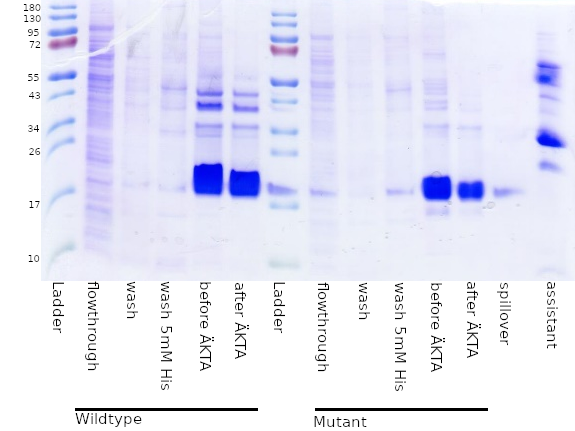
\includegraphics[width=\textwidth]{../img/sds_wt_mut}
	\caption{SDS PAGE gel of \hs{} and \hsmut{}}
        \label{fig:sds_wt_mut}
    \end{subfigure}
    ~
    \begin{subfigure}{0.45\textwidth}
        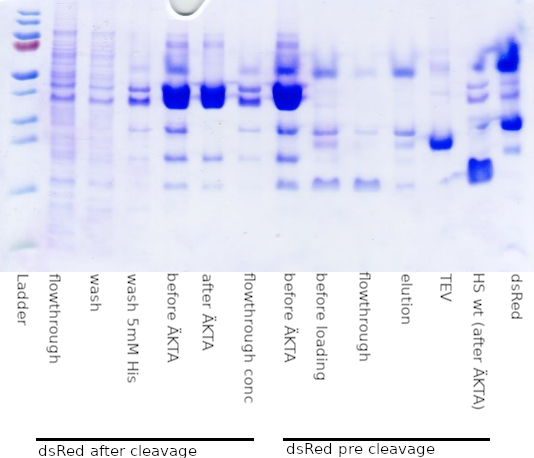
\includegraphics[width=\textwidth]{../img/sds_dsred_tev_cleavage.png}
	\caption{SDS PAGE gel of \hsdsred{} including cleaved \hsdsred{}}
        \label{fig:sds_dsred_cleaved}
    \end{subfigure}
    \caption{SDS gels of three protein variants}
    \label{fig:sds}
\end{figure*}

\subsection{Purification efficiency}

Fluorescence values of \hsdsred{} samples, from aliquots taken during various
steps of the purification, scaled to sample volume, are shown in figure
\ref{fig:purification_fluorescence}. They allowed the tracking of losses during
purification steps.

Measurements showed that the breakage of cells in the maximator did not incur
significant losses. Membrane extraction via ultracentrifugation caused
significant losses of protein, as potentially not all membrane proteins had
been pelleted, or parts of the pellets were lost.

Comparison of fluorescence before the \ce{Ni} beads affinity chromatography
(`Membranes') with the one after (`\ce{Ni} beads elution') imply that not a lot
of proteins were lost during affinity chromatography, with the majority of
losses being in the column flowthrough, implying that too much His-tagged
protein was loaded onto the column at once.

Measurements of the reverse IMAC finally confirmed that most of the His-tagged
Dsred which was loaded was able to bind to the column, and was hence found in
the elution.

\begin{figure}
	\centering
	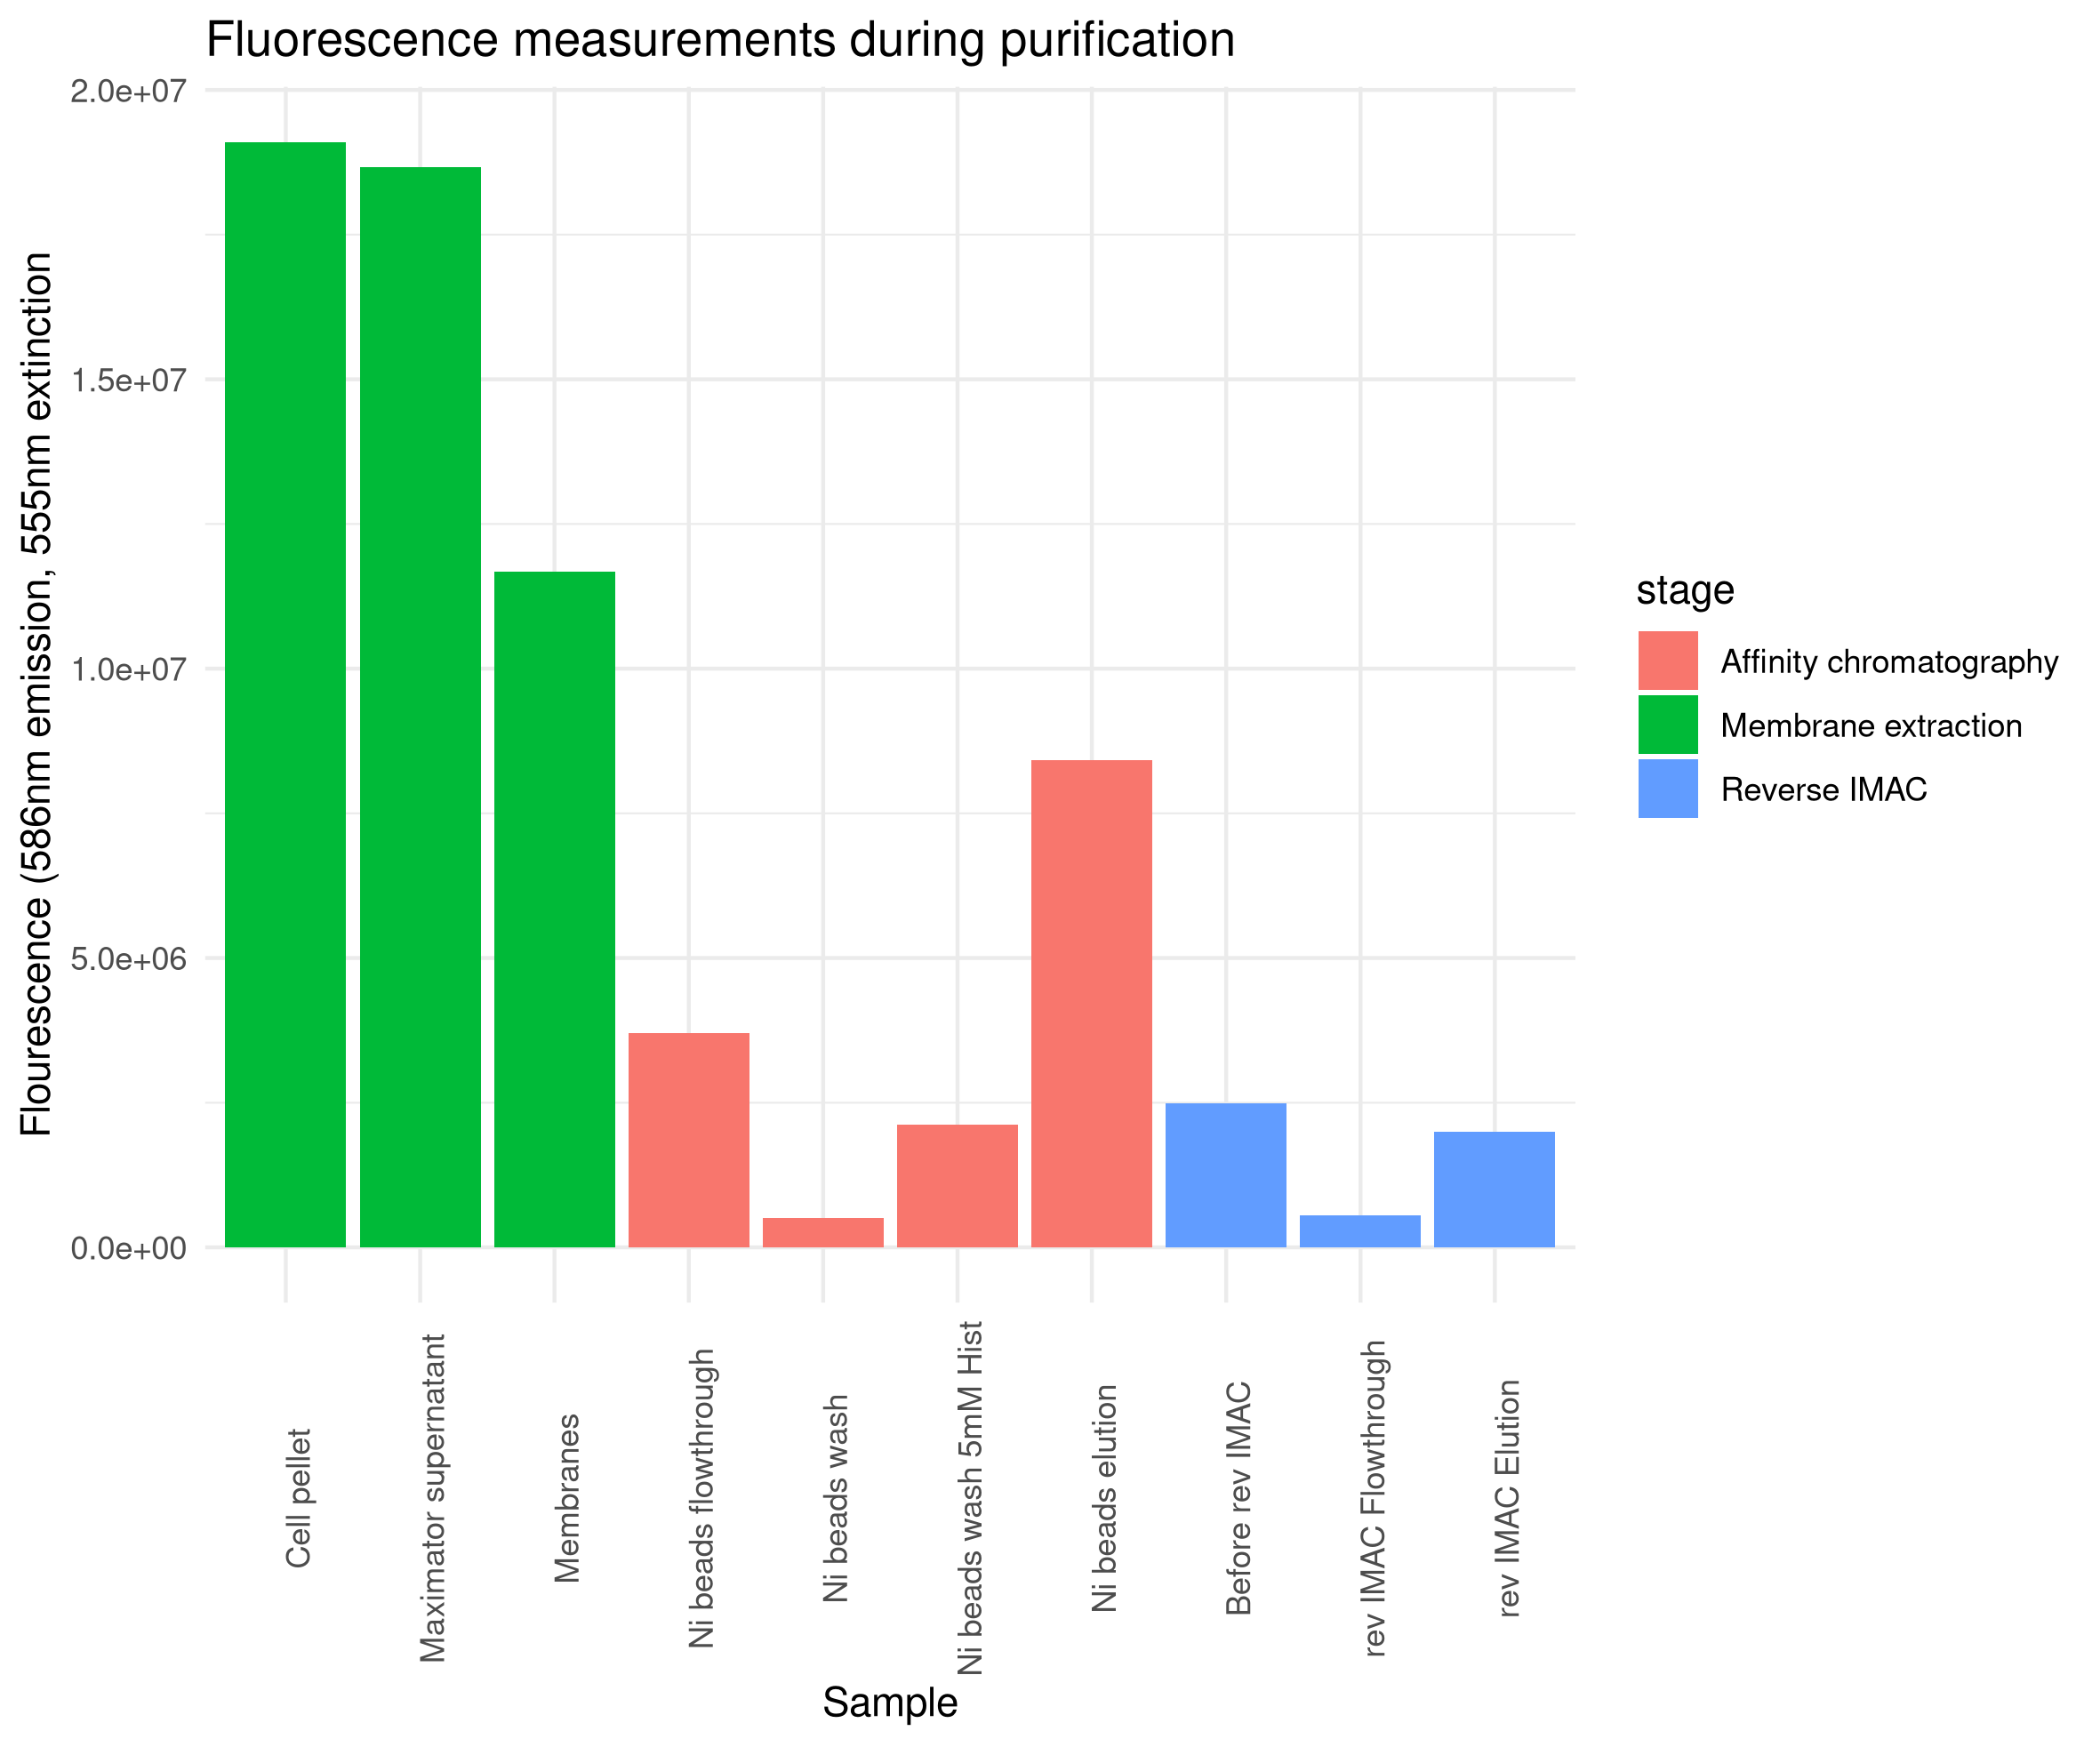
\includegraphics[width=\linewidth]{../img/purification_fluorescence.png}
	\caption{Fluorescence measurements to track purification losses}
	\label{fig:purification_fluorescence}
\end{figure}

\section{Characterization}

The final part of the experiment had the goal to measure relative enzyme
reduction in presence of quinol and superoxide, as well as enzyme activity in a
system containing both.

\subsection{Relative enzyme reduction in presence of quinol \& superoxide}

Absorption measurements of HS as shown in figure \ref{fig:reduction_quinol} and
\ref{fig:reduction_superox} were used to determine the relative reduction rate
of HS in presence of quinol or superoxide. A baseline $od_{\text{base}}$ was
established using the average absorption between \SIrange{0.8}{0.9}{\min}.
Reduction caused by presence of either substrate $od_{\text{substrate}}$ was
determined using the absorption between \SIrange{2.5}{2.6}{\min}, and full
reduction by DTT $od_{\text{full}}$ was determined using absorption between
\SIrange{3.9}{4}{\min}.

% TODO: Table with calculation?
% \begin{table}
% 	\centering
% 	\begin{tabu}{llllll}
% 		\toprule
% 		Protein & State & Baseline & Absorption Quinol & Absorption \SI{100}{\percent} & Rel reduction \\
% 		\midrule
% 		Wildtype & Liposomes & 0.105 & 0.164 & 0.278 & \SI{34}{\percent} \\
% 		Wildtype & Solubilized & 0.092 & 0.130 & 0.304 & \SI{18}{\percent} \\
% 		Mutant & Liposomes & 0.119 & 0.173 & 0.254 & \SI{40}{\percent} \\
% 		Mutant & Solubilized & 0.121 & 0.150 & 0.364 & \SI{12}{\percent} \\
% 		\bottomrule
% 	\end{tabu}
% 	\caption{Relative reduction of HS by quinol addition}
% 	\label{tbl:reduction_quinol}
% \end{table}
Relative reduction rates were calculated as shown in equation
\ref{eq:relative_reduction}, visualized in figures
\ref{fig:reduction_quinol_relative} and \ref{fig:reduction_superox_relative}. 

\begin{equation}
	red_{\text{relative}} := \frac{od_{\text{substrate}} -
	od_{\text{base}}}{od_{\text{full}} - od_{\text{base}}}
	\label{eq:relative_reduction}
\end{equation}

It was shown that the change in absorption was caused by reduction of SOO, as
the addition of DTT to substrate as part of the negative control did not cause
a change in absorption. Further it was shown that superoxide dismutase is able
to effectively quench reduction of superoxide by quickly disproprotionating
superoxide to molecular oxygen and hydrogen peroxide.


\subsubsection{\hs{} vs \hsmut{}}

The data showed no significant difference in relative reduction between \hs{}
and \hsmut{}. This implied that the mutation had no effect on the enzyme
activity if sufficient substrate was present. The mutation might have an effect
on the affinity of the enzyme, lowering enzymatic activity if substrate
concentration is limited, as was shown later.

\subsubsection{Quinol as substrate}

Relative reduction of reconstituted HS was shown to be close to the theoretical
maximum of \SI{50}{\percent}, as only one of the two Hemes can be reduced by
quinol. Relative reduction of solubilized HS was shown to be lower than that of
reconstituted enzymes, which might be the result of hydrophobic quinone binding
to the hydrophobic inner parts of liposomes, which is close to where the active
centre of HS is located\cite{superoxide_salvaging}.

\subsubsection{Superoxide as substrate}

The data shows that the relative reduction of solubilized enzymes by superoxide
is significantly higher than those of reconstituted enzymes. This might imply
that superoxide is unable to enter liposomes, such that in the case of
liposomes it cannot reduce those HS enzymes whose superoxide-oxidating site is
within the liposome. Such an observation was also made in the one of the
referenced papers \cite{superoxide_salvaging}. If this holds then the ratio of
HS oriented such that the superoxide-oxidating end is on the outside of the
liposomes can be estimated to be about half the total amount of reconstituted
HS.

\begin{figure*}
    \centering
    \begin{subfigure}{0.45\textwidth}
	\centering
	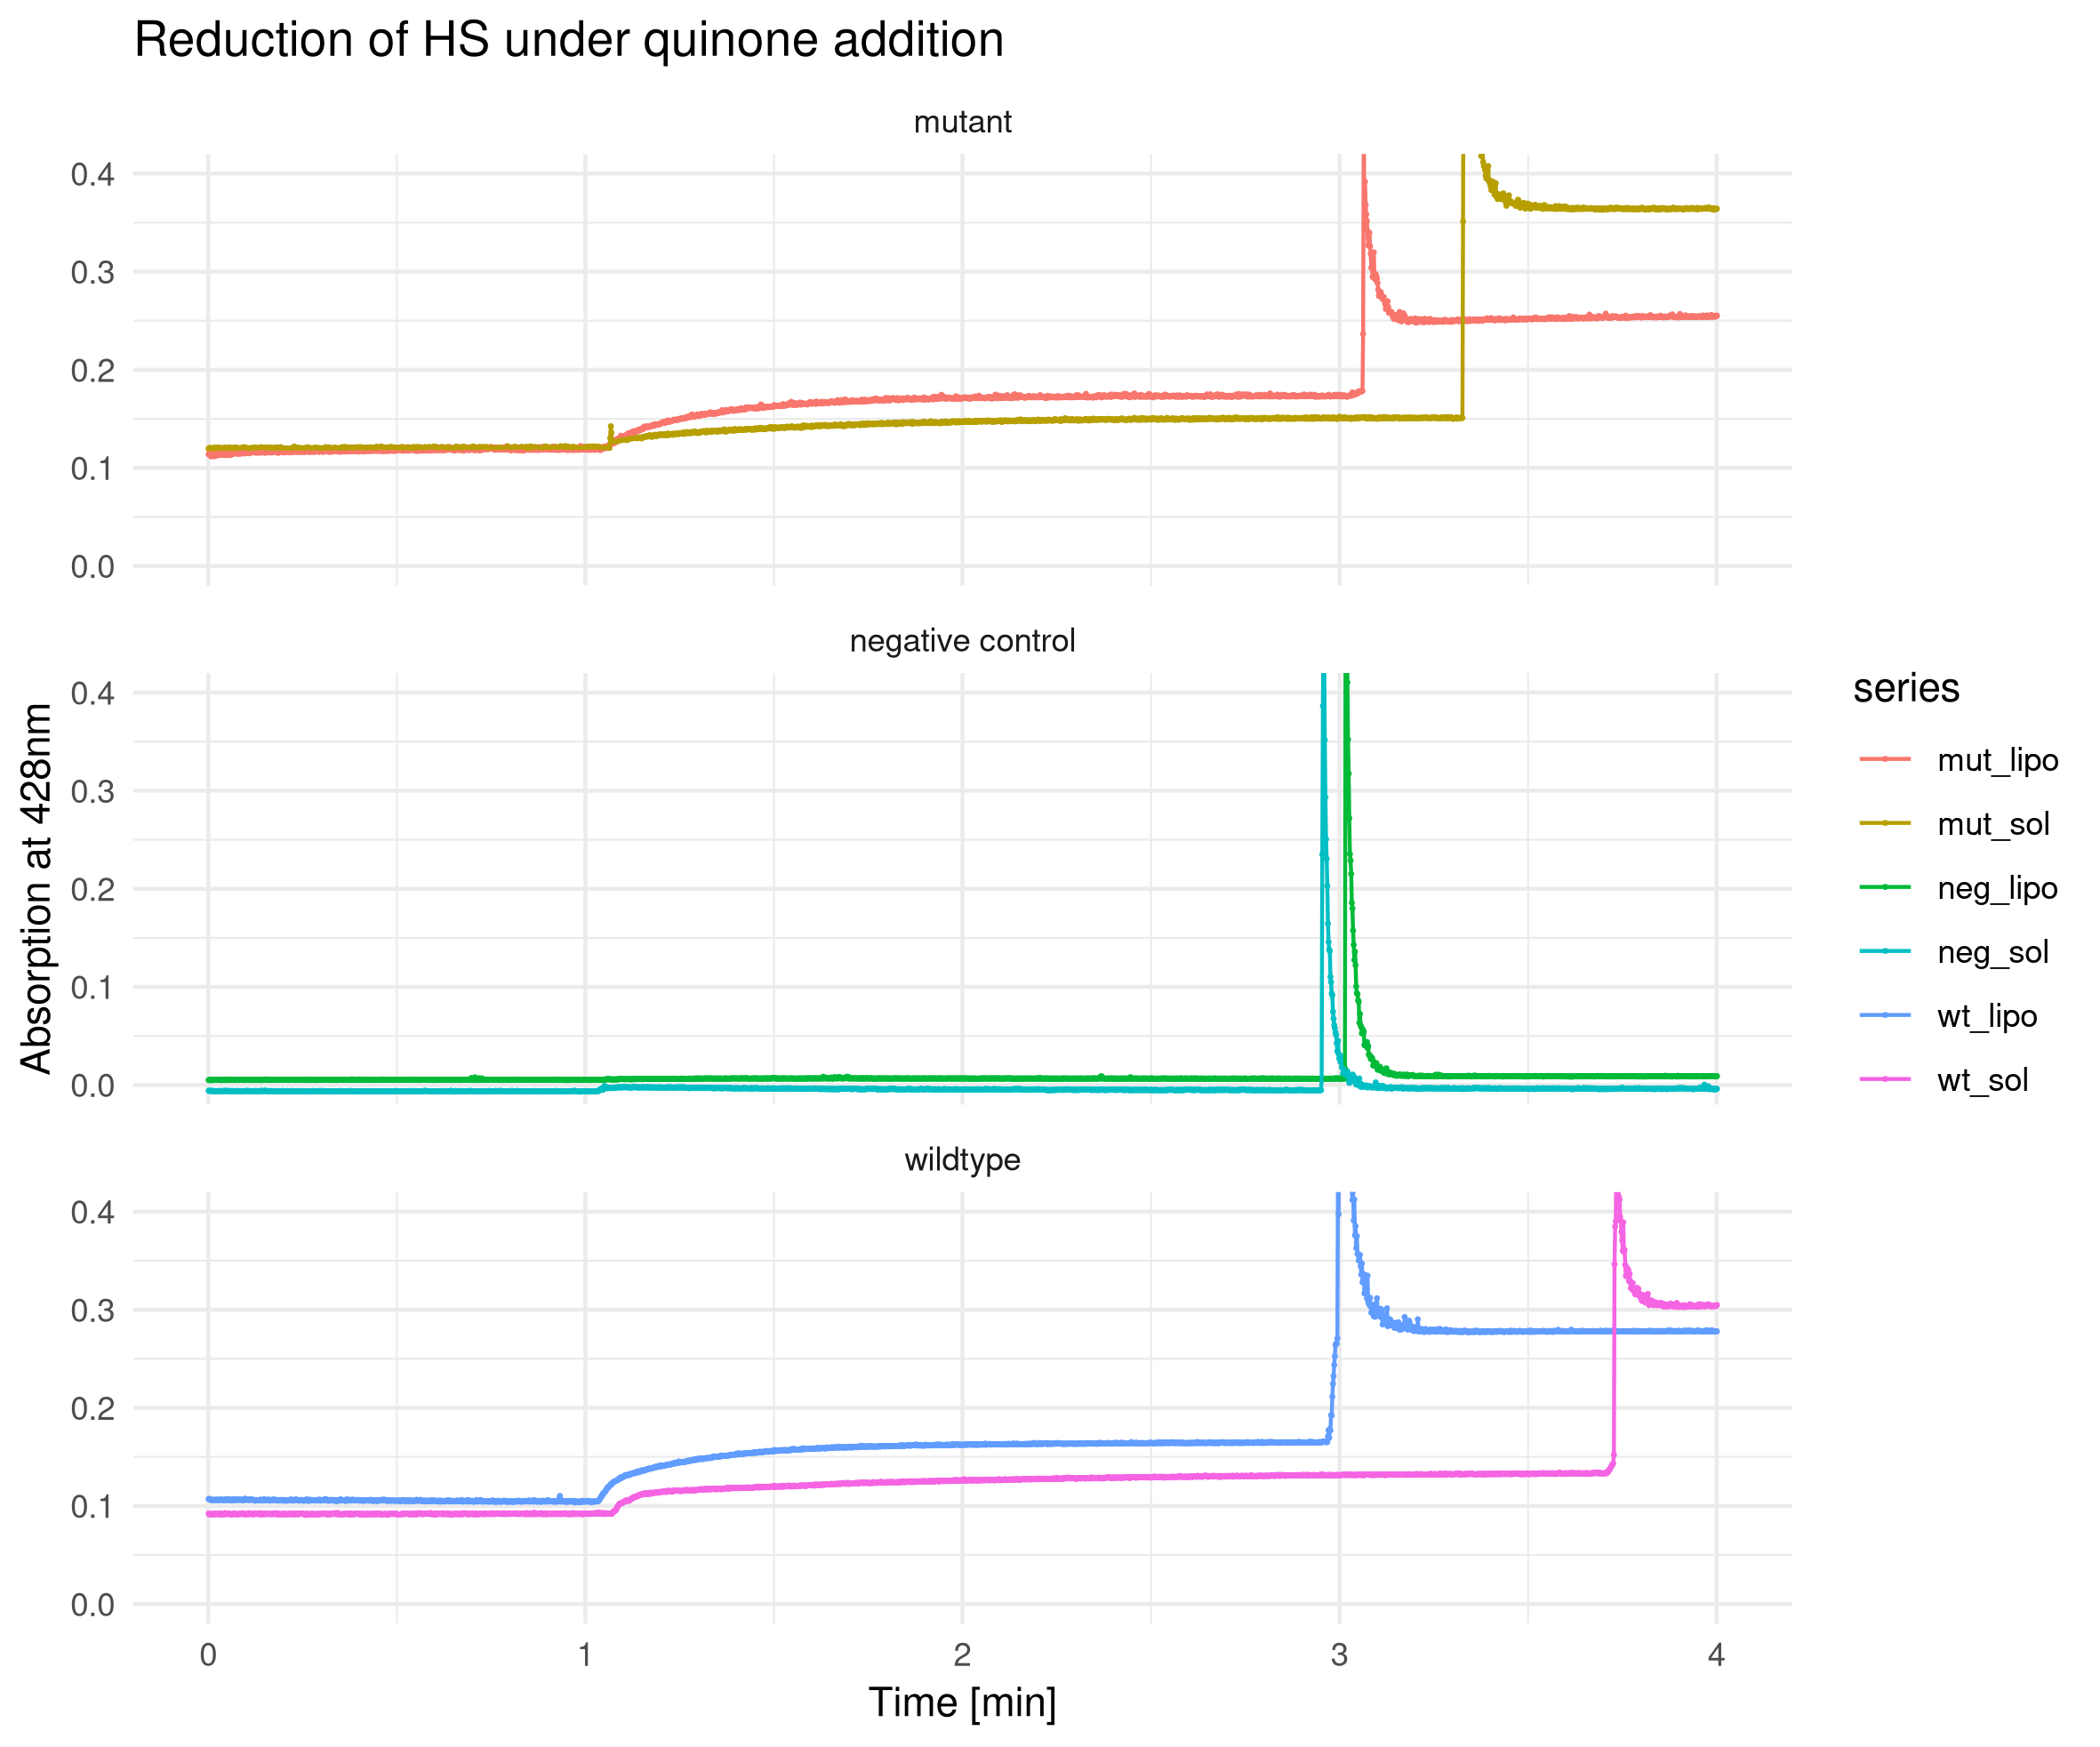
\includegraphics[width=\textwidth]{../img/reduction_quinol.png}
	\caption{Reduction of HS by quinol}
	\label{fig:reduction_quinol}
    \end{subfigure}
    ~
    \begin{subfigure}{0.45\textwidth}
	\centering
	\includegraphics[width=\textwidth]{../img/reduction_superox.png}
	\caption{Reduction of HS by superoxide}
	\label{fig:reduction_superox}
    \end{subfigure}

    \begin{subfigure}{0.45\textwidth}
	\centering
	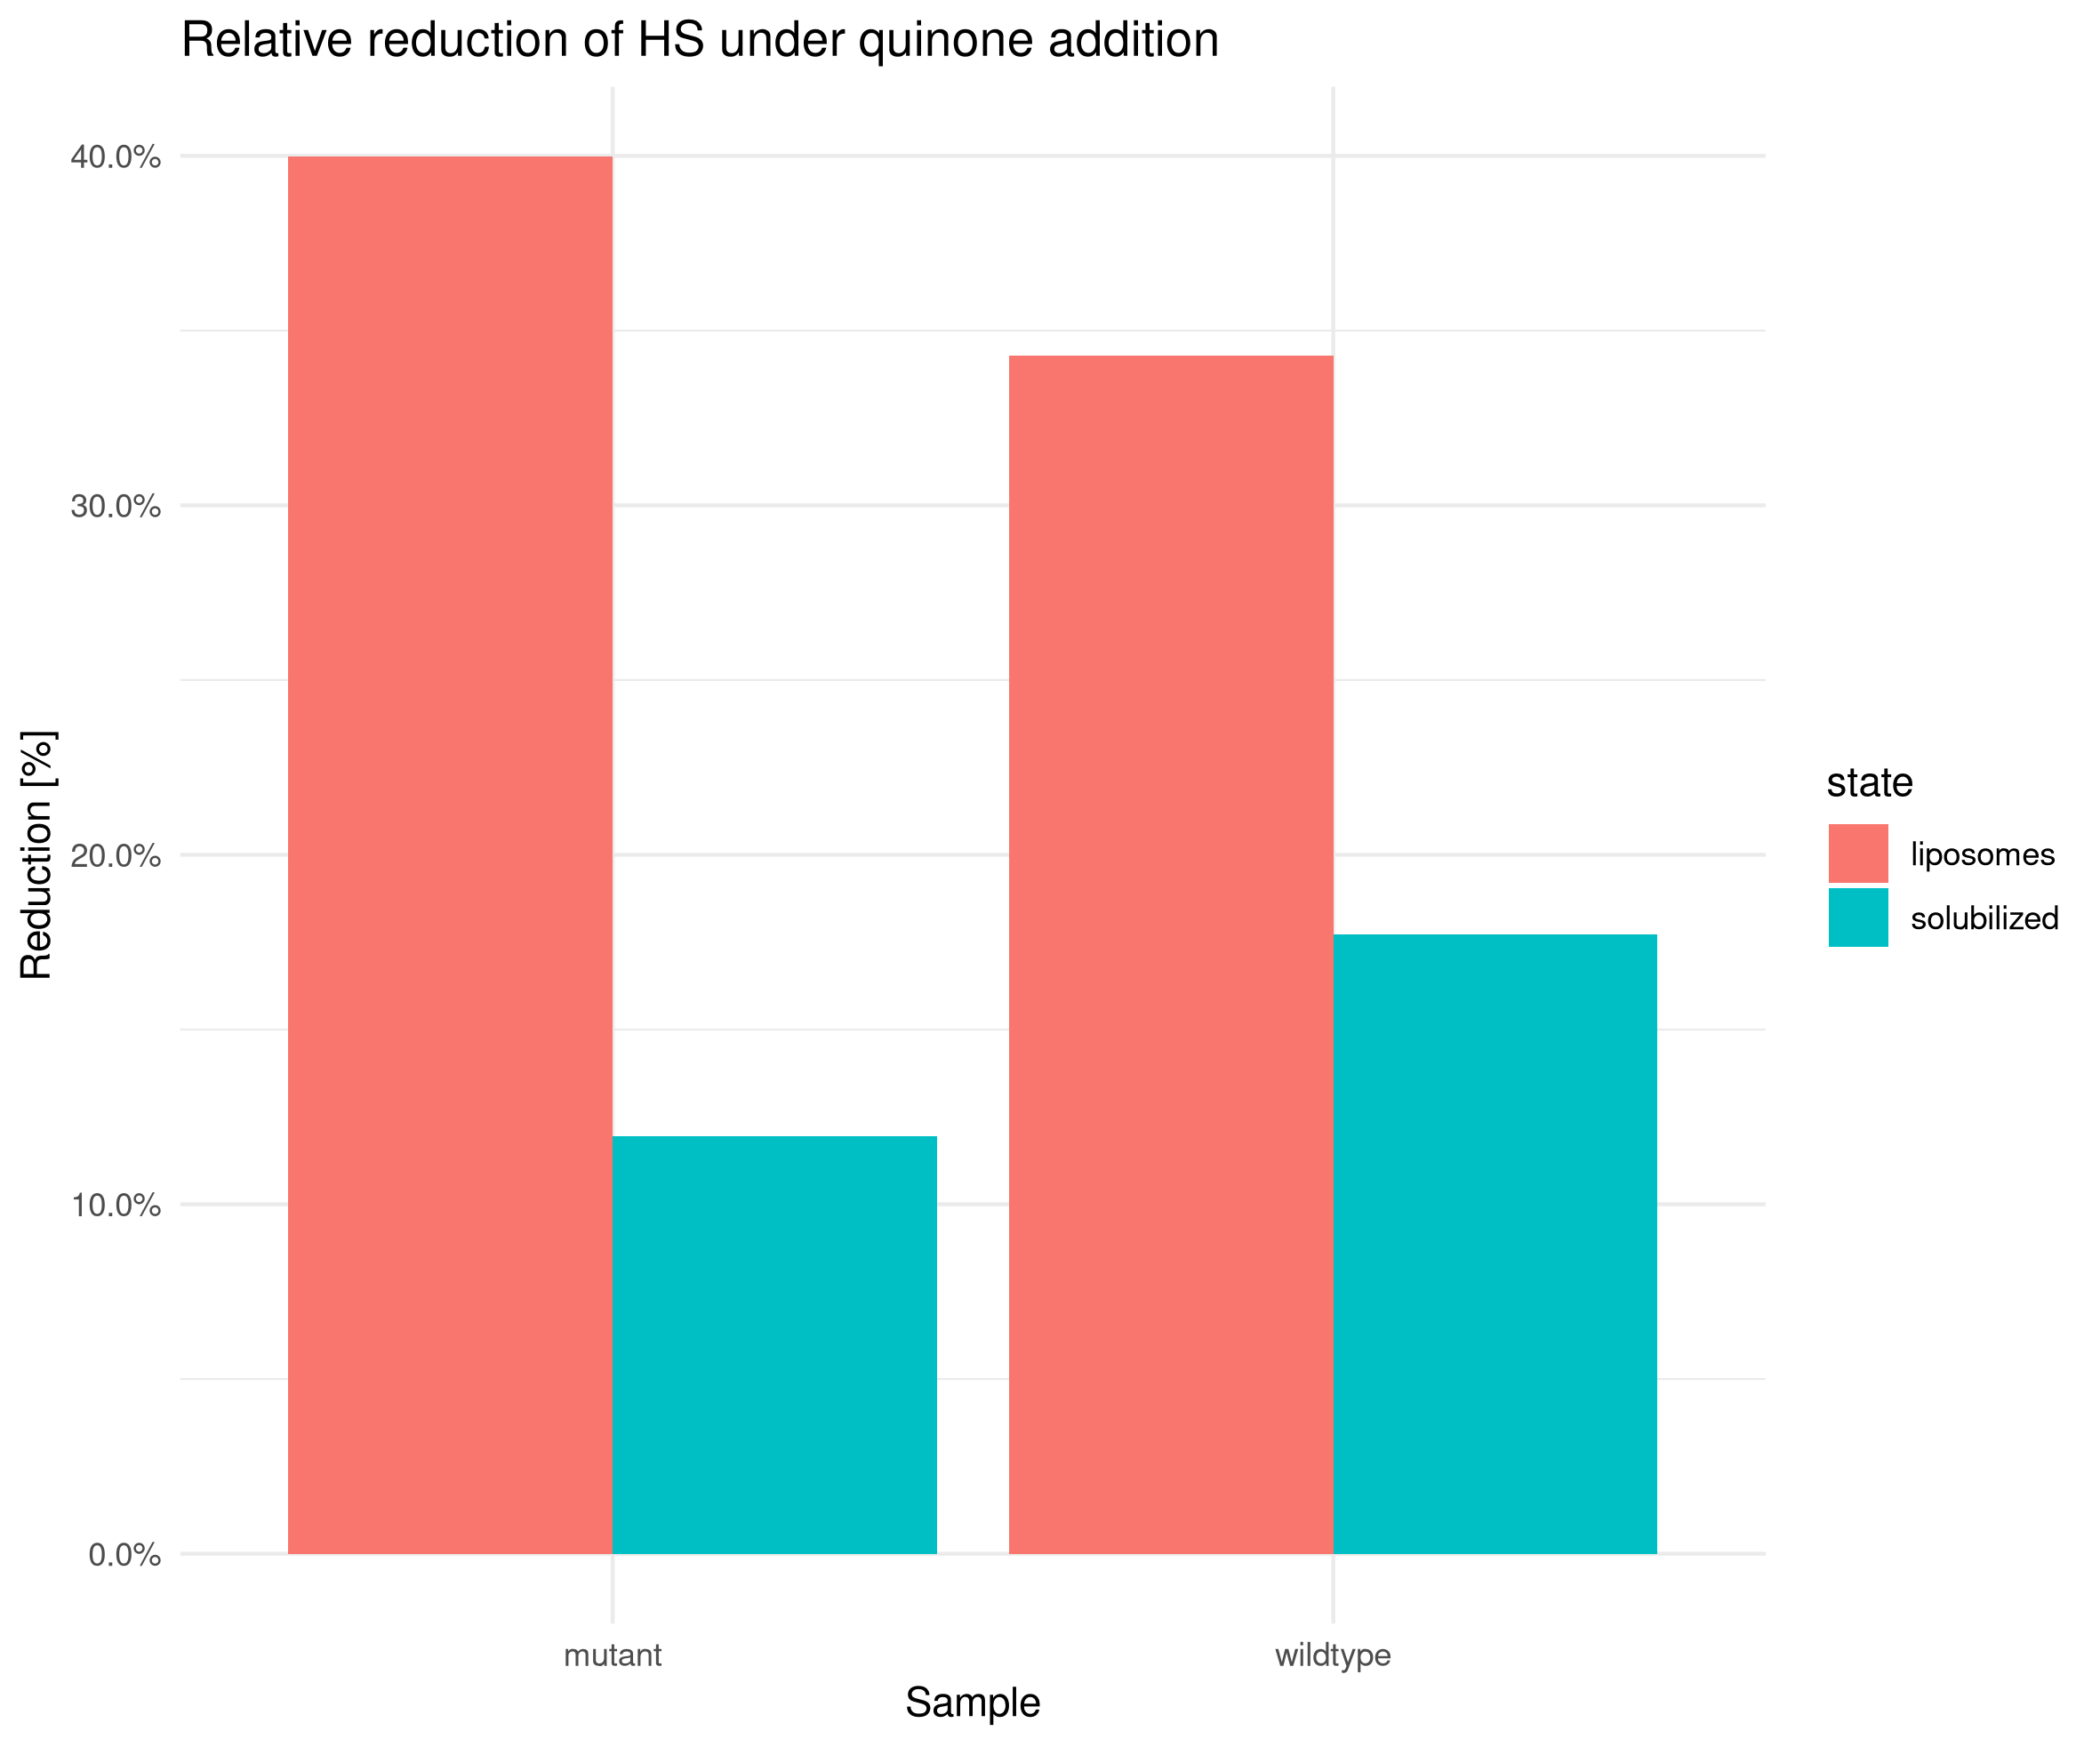
\includegraphics[width=\textwidth]{../img/reduction_quinol_relative.png}
	\caption{Relative reduction of HS by quinol}
	\label{fig:reduction_quinol_relative}
    \end{subfigure}
    ~
    \begin{subfigure}{0.45\textwidth}
	\centering
	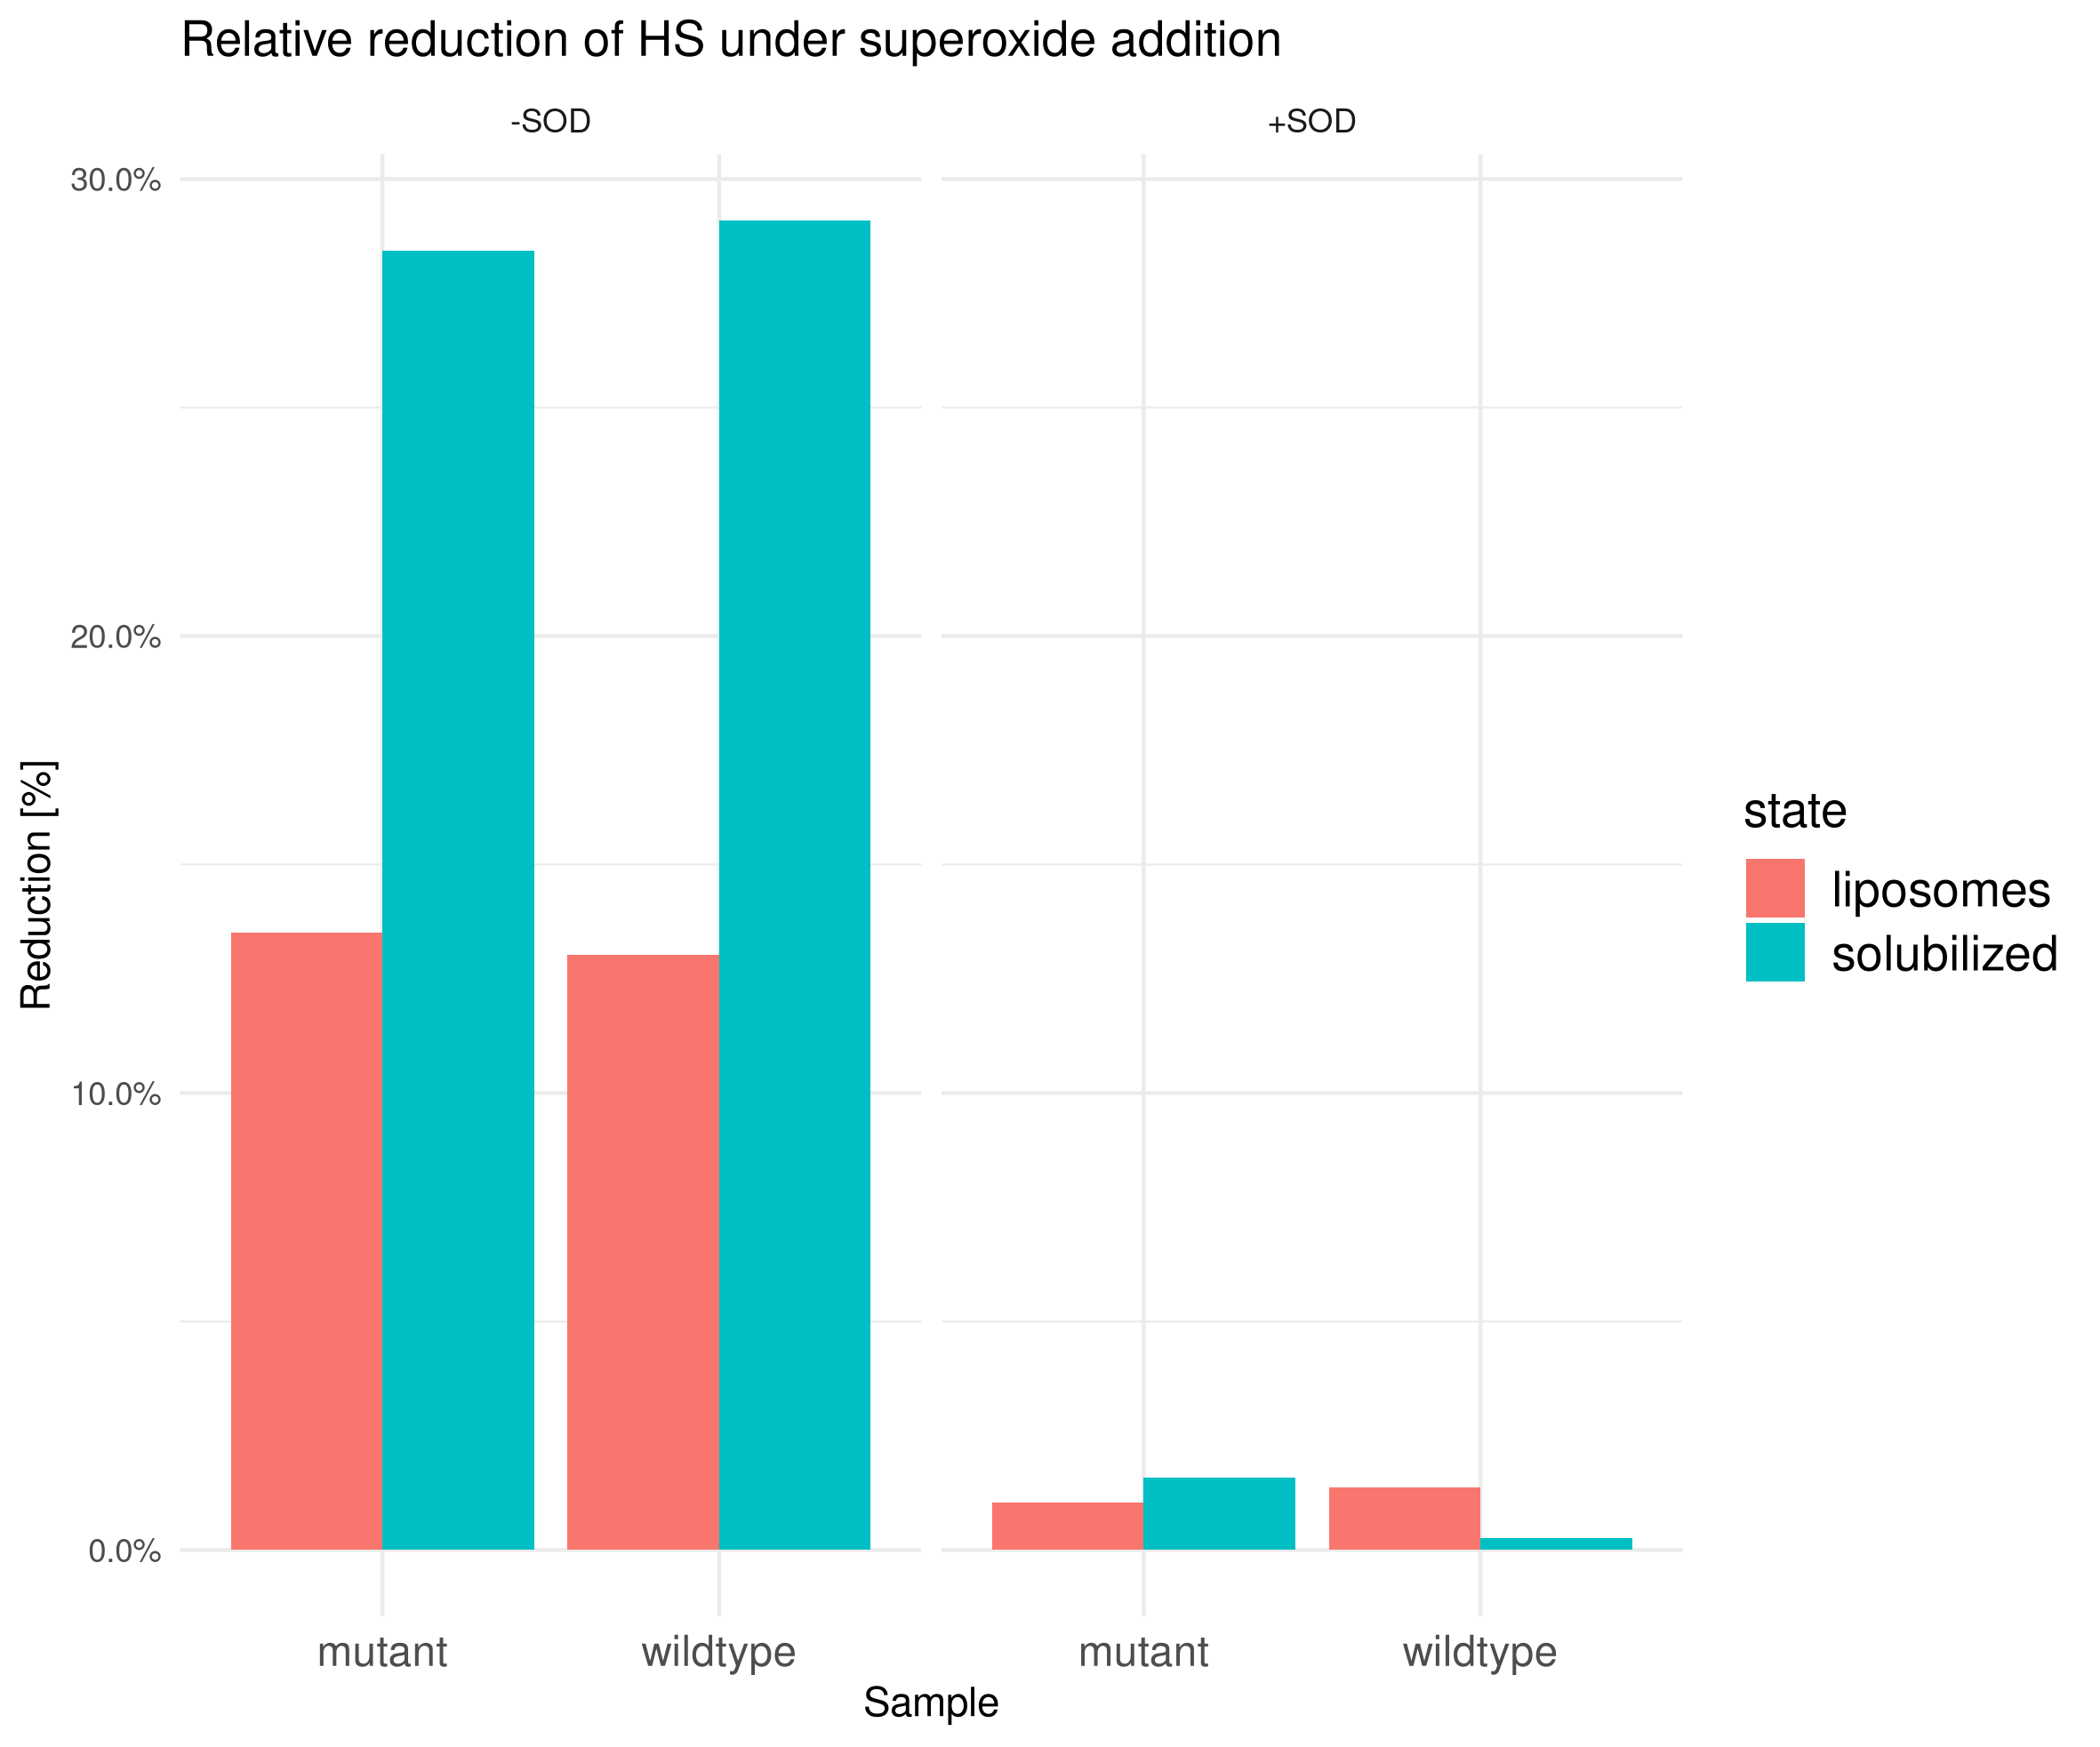
\includegraphics[width=\textwidth]{../img/reduction_superox_relative.png}
	\caption{Relative reduction of HS by superoxide}
	\label{fig:reduction_superox_relative}
    \end{subfigure}
    \caption{Reduction of HS by substrates}
    \label{fig:hs_reduction}
\end{figure*}

% TODO table with relative reduction rates?

\subsection{Fluorescence before and after TEV cleavage of reconstituted enzymes}

To control whether overnight TEV-cleavage was successful, fluorescence of
cleaved and uncleaved reconstituted liposomes with \hsmut{} was measured.
Furthermore the ability to quench and restore fluorescence via addition of
\SI{1}{\milli\Molar} \ce{Cu^{2+}} and \SI{10}{\milli\Molar} EDTA respectively
was investigated. Collected data is shown in figure
\ref{fig:dsred_cleavage_fluorescence}.

The sample with solubilized measurement showed that the method of quenching
Dsred fluorescence with copper, and restoring it via addition of the chelating
agent EDTA, works

It was shown that fluorescence of reconstituted liposomes with \hsdsred{} was
able to be quenched similarly, with nearly complete quenching for sufficiently
high copper concentrations in relation to liposome concentration. This implied
that the liposome contained \hsdsred{} orientated such that Dsred is on the
outside of the liposomes, where copper was able to reach it. The not quite
complete quenching implies that either not enough copper had been added, or
that some \hsdsred{} was oriented such that its Dsred is on the inside of the
liposome. Further experiments with increased copper concentration would be
needed to bring clarity.

Similarly fluorescence of cleaved liposomes was able to be quenched via
addition of copper and restored with EDTA. This implied that uncleaved
\hsdsred{} had remained facing the outside of the liposomes, so cleavage had
not been complete, or that small amounts of cleaved Dsred had remained in the
supernatant after ultracentrifugation.

While initial fluorescence of uncleaved reconstituted liposomes with \hsdsred{}
was higher than that of TEV-treated ones, this allowed no direct conclusion on
whether TEV cleavage was successful, as the concentration of TEV-treated vs
untreated liposomes had not been standardised.

\begin{figure}
	\centering
	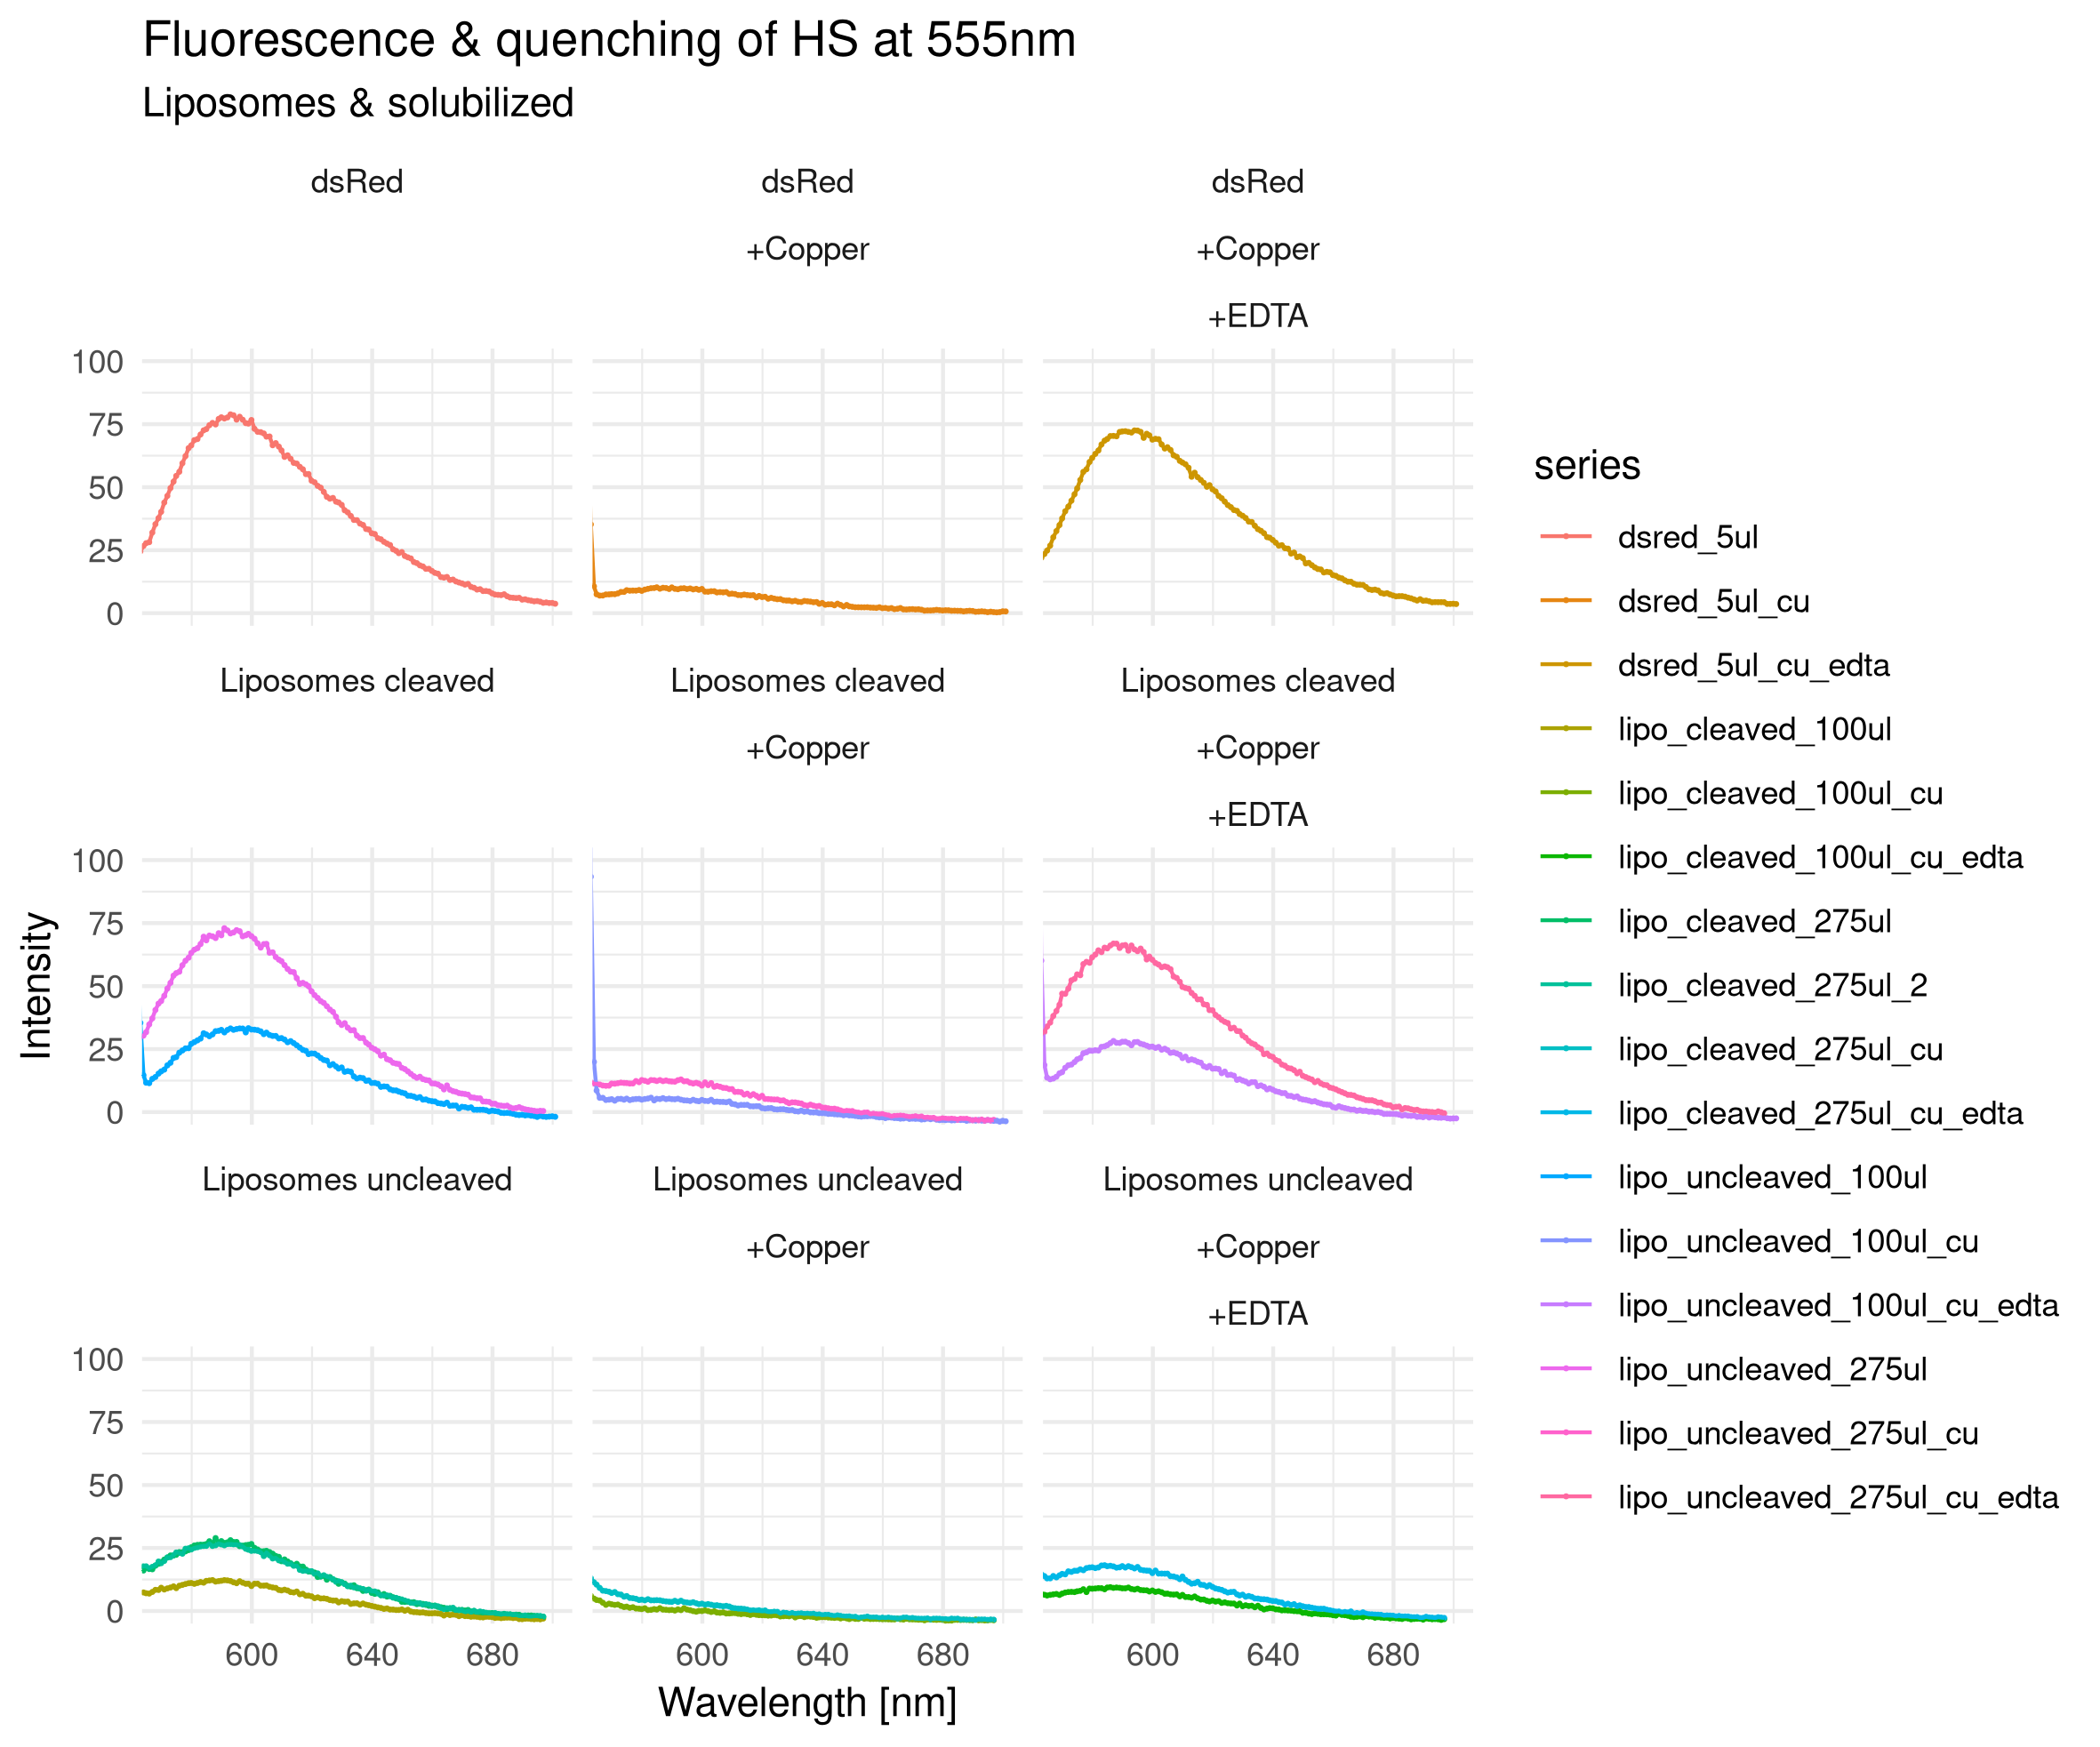
\includegraphics[width=\linewidth]{../img/dsred_cleavage_fluorescence.png}
	\caption{Fluorescence and quenching thereof of cleaved and uncleaved reconstituted liposomes with \hsdsred{}}
	\label{fig:dsred_cleavage_fluorescence}
\end{figure}

\subsection{Enzyme activity}

In order to determine enzymatic activity an assay containing a source of
superoxide (xanthine oxidase and hypoxanthine), a source of quinone (quinone
and BO3 oxidase), and WST-1 dye to measure superoxide concentration via
absorption measurement at \SI{455}{\nm} was used.

In a first step, sufficient HS concentration to quench superoxide production as
efficiently as SOD was determined, which was \SI{4.764}{\micro\Molar} for 
\hsmut{}, \SI{0.496}{\micro\Molar} for \hs{}.

In a second step the concentration of superoxide via WST-1 reduction was
observed. As before the system was prepared and measurements started. XO and HS
were added with a delay, three slopes were measured:

\begin{itemize}
	\item $s_{\text{HS}}$: Slope after HS addition
	\item $s_{\text{XO}}$: Average slope after XO addition
	\item $s_{\text{SOD}}$: Slope after SOD addition
\end{itemize}

This allowed calculating the relative superoxide production as
$\text{SO}_{\text{rel}} := \frac{s_{\text{HS}}}{s_{\text{XO}} -
s_{\text{SOD}}}$ , and relative reduction of superoxide - corresponding to
enzymatic activity - as  $\text{HS-Activity}_{\text{rel}} := 1 -
\text{SO}_{\text{rel}}$. Such results in a linear as well as double-reciprocal
Lineweaver-Burke plot are shown in figures \ref{fig:activity_km} and
\ref{fig:activity_km_lb}.

A linear regression $y = a \cdot x + b$ was performed on the Lineweaver-Burke
plot. Using those parameters the maximum reaction velocity and $K_m$ were
determined as $v_\text{max} := b^{-1}$, $K_m := v_\text{max} \cdot a$.
Calculated values are shown in table \ref{tbl:activity_km}. It was shown that
the $K_m$ of \hsmut{} was two two three orders of magnitude lower than that
of \hs{}, implying that the mutation either lowered the affinity of the
enzyme for its substrate, or decreased the speed at which they are processed.

\begin{figure}
	\centering
	\begin{subfigure}{\linewidth}
		\centering
		\includegraphics[width=\linewidth]{../img/activity_km.png}
		\caption{Relative activity}
		\label{fig:activity_km}
	\end{subfigure}
	\\
	\begin{subfigure}{\linewidth}
		\centering
		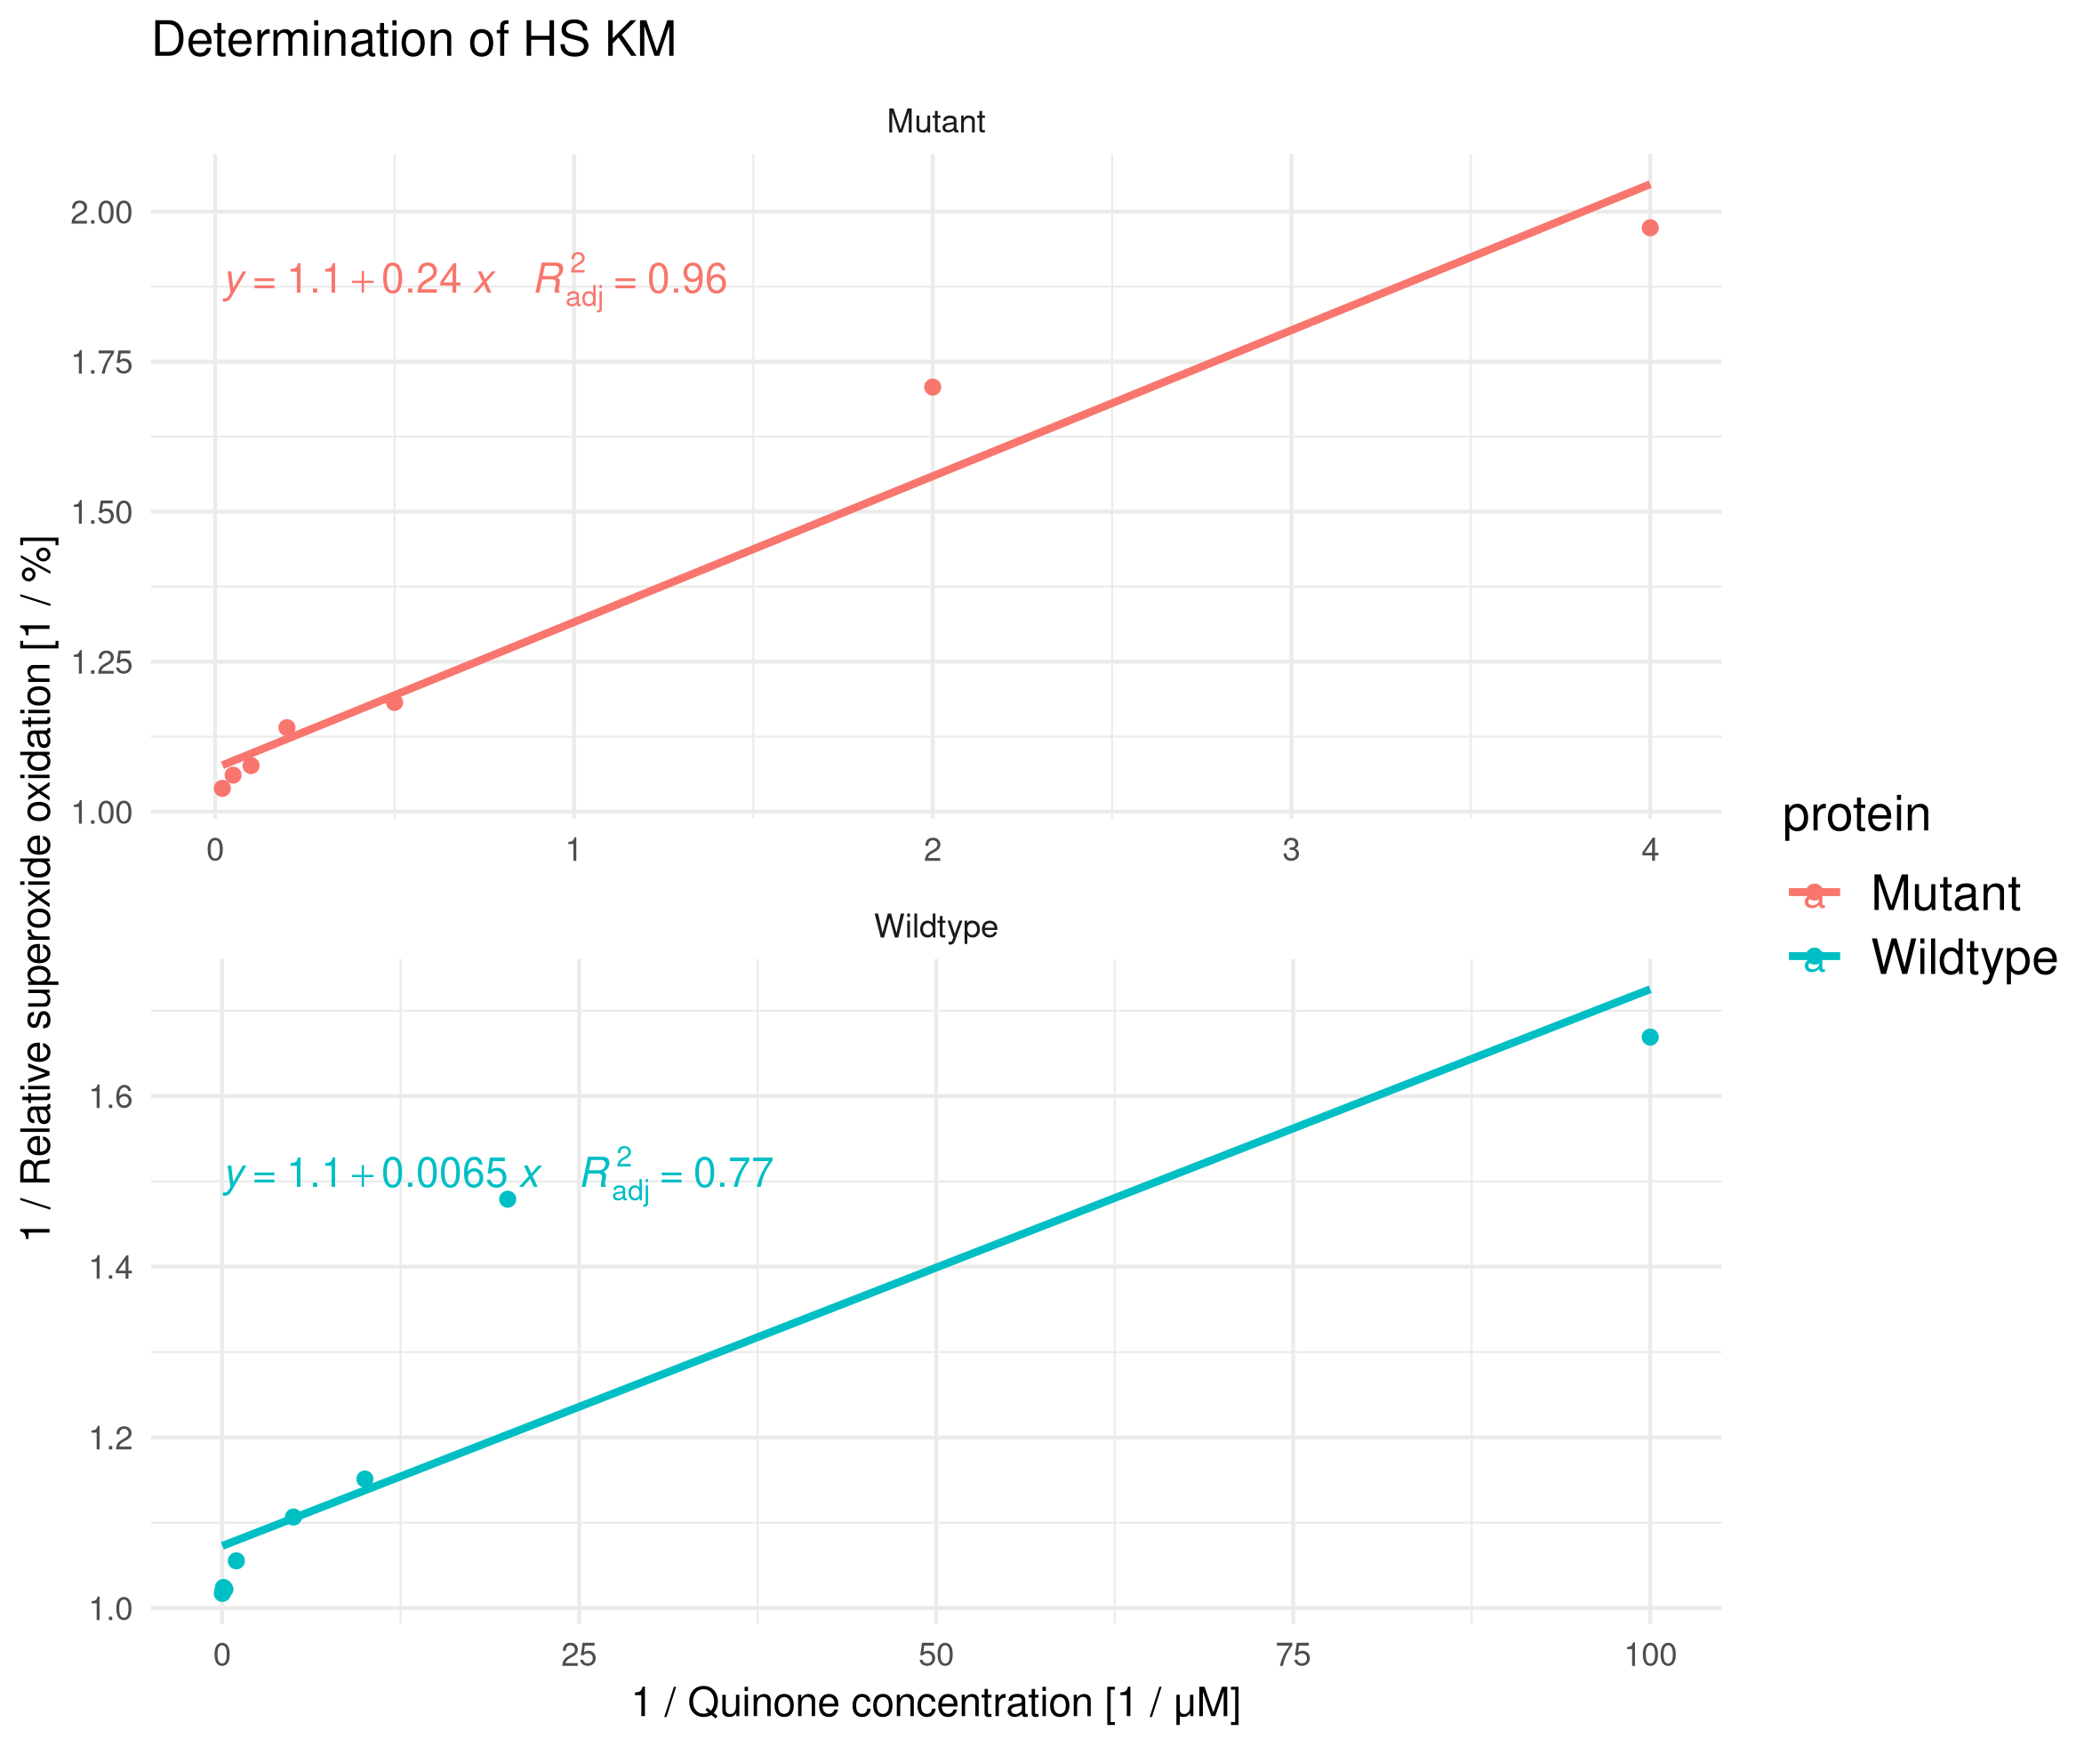
\includegraphics[width=\linewidth]{../img/activity_km_lb.png}
		\caption{LB plot of activity}
		\label{fig:activity_km_lb}
	\end{subfigure}

	\caption{Activity determination of \hs{} \& \hsmut{}}
	\label{fig:activity}
\end{figure}

\begin{table}
	\centering
	\begin{tabu}{l|ll}
		\toprule
		Protein & \hs{} & \hsmut{} \\
		Slope $a$ & 0.0065 & 0.24 \\
		Y-intercept $b$ & 1.1 & 1.1 \\
		$v_{\text{max}} = b^{-1}$ & \SI{90.9}{\percent} & \SI{90.9}{\percent} \\
		$K_m = v_{\text{max}} \cdot a$  & \SI{0.0059}{\micro\Molar} & \SI{0.218}{\micro\Molar} \\
		\bottomrule
	\end{tabu}
	\caption{Determination of $K_m$ for HS}
	\label{tbl:activity_km}
\end{table}



\part{Conclusion}

\section{Summary of results}

In this work it was shown that membrane protein yield per call can be increased
by using ZYM-505 auto-induction medium. Further it was shown that superoxide
oxidase can be purified reasonably well using an affinity and size exclusion
chromatography after extraction of membranes.

It was shown that cybB561 is able to be reduced by both superoxide as well as
quinol, confirming that these two are valid substrates. Its $K_m$ with relation
to quinone concentration was determined, with a difference of two to three
orders of magnitude between \hs{} and \hsmut{}.

Lastly evidence was found implying that SOO reconstituted into liposomes can
take on both orientations.

\section{Protein expression \& purification}

Being able to achieve a higher yield of membrane proteins allows to
significantly increase the amount of expressed and hence purified protein,
without increasing the requirement for potentially expensive detergent caused
by an increase in number of cells, as would be the result of expression in
TB.\cite{memstar}

Purification results showed that a reasonably pure product could be achieved in
a relatively short amount of time, using readily-available methods. It further
provided information on which steps of purification should be adjusted to
prevent losses, such as ensuring that no protein is lost in the flowthrough of
affinity chromatography.

The ability of rhamnose to slightly inhibit the T7 polymerase, helping to
prevent the buildup of inclusion bodies, could not be observed as expected. A
further attempt of the expression screening part of the experiment should be
made to bring clarity.
\section{Enzyme activity}

CybB is known as an extremely fast, diffusion-limited
enzyme.\cite{superoxide_salvaging}. The difference in $K_m$ values of \hsmut{}
and \hs{} implied that the conserved Histidine played a role in the binding of,
or reaction with, substrate.

Additional measurements with lower quinone concentration would allow to more
accurately determine the $K_m$ value.

\section{Membrane protein orientation}

The seemingly non-uniform orientation of HS in liposomes - as opposed to in
vivo where orientation is uniform - is of importance for experiments wanting to
use HS as part of a system modelling parts of the respiratory chain.

A clearer picture could be gathered by repeating cleavage and fluorescence
measurements, taking care to incubate long enough that cleavage would be
complete, as well as adding enough copper to quench fluorescence completely.



\newpage
\bibliographystyle{plain}
\bibliography{references}

\end{document}
